%%% The ``\documentclass'' command has one parameter, based on the kind of
%%% document you are preparing.
%%%
%%% [annual] - Technical paper accepted for presentation at the ACM SIGGRAPH
%%%   or SIGGRAPH Asia annual conference.
%%% [sponsored] - Short or full-length technical paper accepted for
%%%   presentation at an event sponsored by ACM SIGGRAPH
%%%   (but not the annual conference Technical Papers program).
%%% [abstract] - A one-page abstract of your accepted content
%%%   (Technical Sketches, Posters, Emerging Technologies, etc.).
%%%   Content greater than one page in length should use the "[sponsored]"
%%%   parameter.
%%% [preprint] - A preprint version of your final content.
%%% [review] - A technical paper submitted for review. Includes line
%%%   numbers and anonymization of author and affiliation information.

\documentclass[annual]{acmsiggraph}

\usepackage{amsmath}
\usepackage{amssymb}
\usepackage{amsthm}
\usepackage{par06}
\usepackage{overpic}
\usepackage{contour}\contourlength{1pt}
\usepackage{color}

\long\def\nix#1{\relax}


\def\div{\DID YOU RELLY WANT TO USE \div?}
\def\<{\mathchoice{\big\langle}{\langle}{\langle}{\langle}}
\def\>{\mathchoice{\big\rangle}{\rangle}{\rangle}{\rangle}}
%\def\lll{\mathopen{\mbox{$\<\hskip-.5ex\<$}}}
%\def\rrr{\mathclose{\mbox{$\>\hskip-.5ex\>$}}}
\def\wh{\widehat}
%\def\II{\mbox{I\hskip-0.1exI}}
\newtheorem{theorem}{Theorem}
\newtheorem{prop}[theorem]{Proposition}
\def\Div{\mathop{{\rm div}}\nolimits}
\def\tr{\mathop{{\rm tr}}\nolimits}
\def\rel{{\mathord{{\rm rel}}}}
\def\const{{\mathord{\textrm{const}}}}
\def\ess{s}
\def\Hess#1{{\def\testess{#1}\nabla^2\ifx\testess\ess\!s\else #1\fi}}
\def\Hess#1{\text{$\nabla^2\hskip-.2ex #1$}}
\def\Forcevector{\Big(\mbox{\scriptsize
	\def\arraystretch{0.8}\begin{tabular}{@{\,}c@{\,}}
	0 \\ 0 \\ $A_i F_i$
	\end{tabular}}\Big)}
\hyphenation{pa-rab-ol-loid War-detz-ky}

\def\lput(#1,#2)#3{\put(#1,#2){\hbox to 0pt{\hss{#3}}}}
\def\cput(#1,#2)#3{\put(#1,#2){\hbox to 0pt{\hss{#3}\hss}}}
\definecolor{blau}{rgb}{0.15,0.2,0.3}
%\definecolor{rot}{rgb}{0.7,0.5,0.2}
\definecolor{drot}{rgb}{0.7,0,0.1}
\definecolor{grey}{rgb}{0.6,0.6,0.6}
\definecolor{lightgrey}{rgb}{0.8,0.8,0.8}
\definecolor{gelb}{rgb}{.55,.40,.1}


\outer\def\proclaim #1. #2\par{\noindent{\bf#1.\enspace}{\it#2\par}}


%\usepackage{mathrsfs}
\def\SS{{\mathcal S}}
\def\RR{{\mathcal R}}

\newcommand{\newtext}[1]{\textcolor{red}{#1}}
\newcommand{\todo}[1]{\textcolor{red}{#1}}
\newcommand{\secref}[1]{(\S\ref{#1})}

%%% If you are submitting your paper to one of our annual conferences - the
%%% ACM SIGGRAPH conference held in North America, or the SIGGRAPH Asia
%%% conference held in Southeast Asia - there are several commands you should
%%% consider using in the preparation of your document.

%%% 1. ``\TOGonlineID''
%%% When you submit your paper for review, please use the ``\TOGonlineID''
%%% command to include the online ID value assigned to your paper by the
%%% submission management system. Replace '45678' with the value you were
%%% assigned.

\TOGonlineid{0043}

%%% 2. ``\TOGvolume'' and ``\TOGnumber''
%%% If you are preparing a preprint of your accepted paper, and your paper
%%% will be published in an issue of the ACM ``Transactions on Graphics''
%%% journal, replace the ``0'' values in the commands below with the correct
%%% volume and number values for that issue - you'll get them before your
%%% final paper is due.

\TOGvolume{0}
\TOGnumber{0}

%%% 3. ``TOGarticleDOI''
%%% The ``TOGarticleDOI'' command accepts the DOI information provided to you
%%% during production, and which makes up the URLs which identifies the ACM
%%% article page and direct PDF link in the ACM Digital Library.
%%% Replace ``1111111.2222222'' with the values you are given.

\TOGarticleDOI{1111111.2222222}

%%% 4. ``\TOGprojectURL'', ``\TOGvideoURL'', ``\TOGdataURL'', ``\TOGcodeURL''
%%% If you would like to include links to personal repositories for auxiliary
%%% material related your research contribution, you may use one or more of
%%% these commands to define an appropriate URL. The ``\TOGlinkslist'' command
%%% found just before the first section of your document will add hyperlinked
%%% icons to your document, in addition to hyperlinked icons which point to
%%% the ACM Digital Library article page and the ACM Digital Library-held PDF.

\TOGprojectURL{}
\TOGvideoURL{}
\TOGdataURL{}
\TOGcodeURL{}

%%% Replace ``PAPER TEMPLATE TITLE'' with the title of your paper or abstract.

\title{Design of Self-supporting Surfaces}

%%% The ``\author{}'' command takes the names and affiliations of each of the
%%% authors of your paper or abstract. The ``\thanks{}'' command takes the
%%% contact information for each author.
%%% For multiple authors, separate each author's information by the ``\and''
%%% command.

\author{
	Etienne Vouga
	\\ Columbia Univ. / KAUST
\and
	Mathias H\"obinger
	\\ Evolute / TU Wien
\and
	Johannes Wallner
	\\ TU Graz / TU Wien
\and
	Helmut Pottmann
	\\ KAUST
}

%%% The ``pdfauthor'' command accepts the authors of the work,
%%% comma-delimited, and adds this information to the PDF metadata.

\pdfauthor{Etienne Vouga, Mathias H\"{o}binger, Johannes Wallner, Helmut Pottmann}

%%% Keywords that describe your work. The ``\keywordlist'' command will print
%%% them out.

\keywords{Discrete differential geometry, architectural geometry,
self\dash supporting masonry, thrust networks,
reciprocal force diagrams, discrete Laplacians,
isotropic geometry, mean curvature}

%%% The ``\begin{document}'' command is the start of the document.

%%% If you have user-defined macros, you may include them here.

% example of a user-defined macro called ``remark.''
% \newcommand{\remark}[1]{\textcolor{red}{#1}}

\begin{document}

%%% A ``teaser'' image appears under the title and affiliation information,
%%% horizontally centered, and above the two columns of text. This is OPTIONAL.
%%% If you choose to have a ``teaser'' image, it needs to be placed between
%%% ``\begin{document}'' and ``\maketitle.''

\teaser{\centering
        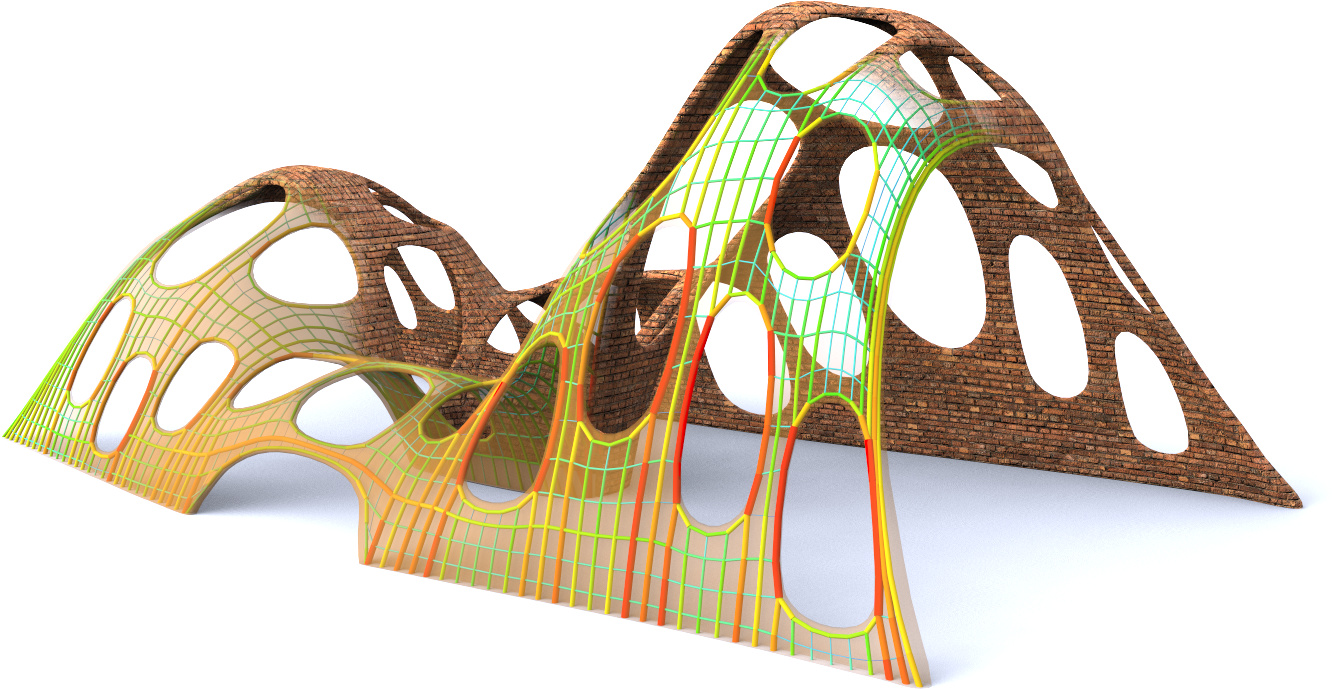
\includegraphics[height=.24\textwidth]{arch-fig/cheesevault78.jpg}
        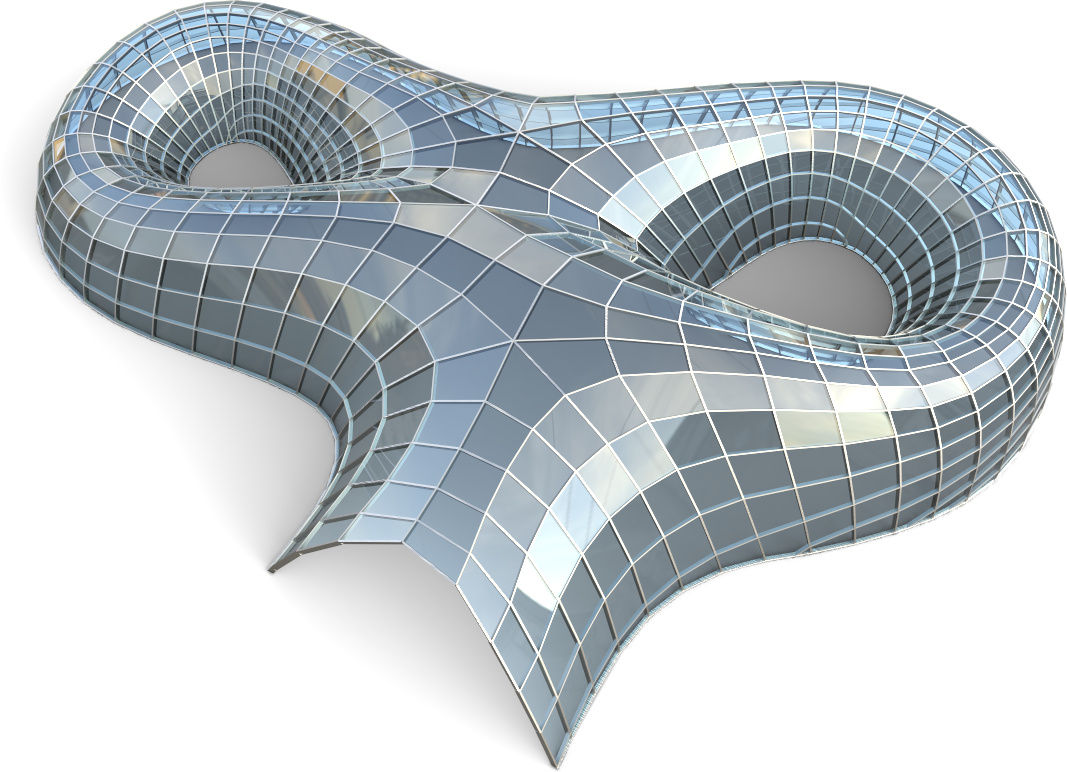
\includegraphics[height=.24\textwidth]{arch-fig/1roo97}

	\caption{{\em Left:} Surfaces with irregularly placed holes
are hard to realize as masonry, where the mortar between bricks
must not be subject to tensile stresses. The surface shown here, surprisingly, has
this property -- it has been found as the nearest
self\dash supporting shape from a given freeform geometry.
The fictitious thrust network used in our algorithms is superimposed, with 
edges' cross-section and coloring visualizing the magnitude of
forces (warmer colors represent higher stresses.)
{\em Right:} Curvature analysis with respect to the
Airy stress surface
tells us how to remesh shapes by self\dash supporting quad meshes
with planar faces. This guides steel\slash glass constructions with
low moments in nodes.}
	\label{fig:teaser}
}

%%% The ``\maketitle'' command must appear after ``\begin{document}'' and,
%%% if you have one, after the definition of your ``teaser'' image, and
%%% before the first ``\section'' command.

\maketitle

%%% Your paper's abstract goes in its own section.

\begin{abstract} Self\dash supporting masonry is one of the most ancient
and elegant techniques for building curved shapes. Because of the
very geometric nature of their failure, analyzing and modeling such strutures
is more a geometry processing problem than
one of classical continuum mechanics. This paper uses the thrust network method
of analysis and presents an iterative nonlinear optimization algorithm for
efficiently approximating freeform shapes by self\dash supporting ones.
The rich geometry of thrust networks leads us to
close connections between diverse topics in discrete differential geometry,
such as a finite\dash element discretization of the Airy stress potential, perfect graph
Laplacians, and computing admissible loads via curvatures of polyhedral
surfaces. This geometric viewpoint allows us, in particular, to remesh self\dash supporting
shapes by self\dash supporting quad meshes with planar faces, and leads
to another application of the theory: steel\slash glass constructions
with low moments in nodes.

\end{abstract}

%%% ACM Computing Review (CR) categories.
%%% See <http://www.acm.org/class/1998/> for details.
%%% The ``\CRcat'' command takes four arguments.

\begin{CRcatlist}
  \CRcat{I.3.5}{Computer Graphics}{Computational Geometry and Object Modeling}{Curve, surface, solid, and object representations};
\end{CRcatlist}

%%% The ``\keywordlist'' command prints out the keywords.

\keywordlist

%%% The ``\TOGlinkslist'' command will insert hyperlinked icon(s) to your
%%% paper. This includes, at a minimum, hyperlinked icons to the ACM article
%%% page and the ACM Digital Library-held PDF. If you added URLs to
%%% ``\TOGprojectURL'' or the other, similar commands, they will be added to
%%% the list of icons.
%%% Note: this functionality only works for annual-conference papers.

\TOGlinkslist

%%% The ``\copyrightspace'' command
%%% Do not remove this command.

\copyrightspace

%%% This is the first section of the body of your paper.

%\insert\footins{\vspace*{4cm}}

\section{Introduction}


Vaulted masonry structures are among the simplest and at the same time
most elegant solutions for creating curved shapes in building
construction. For this reason they have been an object of interest
since antiquity; large, non\dash convex examples of such structures include gothic
cathedrals. They continue to be an active topic of research today.


Our paper is concerned with a combined geometry+statics analysis of {\em
self\dash supporting} masonry and with tools for the interactive modeling
of freeform self\dash supporting structures. Here ``self\dash supporting''
means that the structure, considered as an arrangement of blocks (bricks,
stones), holds together by itself, with additional support present only during
construction. This analysis is based on the following assumptions, which
follow the classic \cite{Heyman66}:


{\it Assumption 1:} Masonry has no tensile strength, but the individual
building blocks do not slip against each other (because of friction or
mortar). On the other hand, their compressive strength is sufficiently
high so that failure of the structure is by a sudden change in geometry
and not by material failure.

{\it Assumption 2 (The Safe Theorem)}: If a system of forces can be found
which is in equilibrium with the load on the structure and which is
contained within the masonry envelope then the structure will carry the
loads, although the actual forces present may not be those postulated by
that system.

Our approach is twofold: We first give an overview of the continuous case
of a smooth surface under stress, which turns out to be governed locally by the
Airy stress function. This mathematical
model is called a membrane in the engineering literature and has been
applied to the analysis of masonry before. The surface is self\dash
supporting if and only if stresses are entirely compressive.
For computational purposes, stresses are
discretized as a fictitious {\em thrust network} \cite{Block07} contained
in the masonry structure; this network is a system of forces in equilibrium with
the structure's deadload. It can be interpreted as a
finite element discretization of the continuous case, and it turns out to
have very interesting geometry, with the Airy stress function becoming a
polyhedral surface directly related to a reciprocal force diagram.

While previous work in architectural geometry was mostly concerned
with aspects of rationalization and purely geometric side\dash conditions
which occur in freeform architecture, the focus of this paper is design with
{\em statics} constraints. In particular, our
contributions are the following:

\nix{
	\begin{figure}[t]
	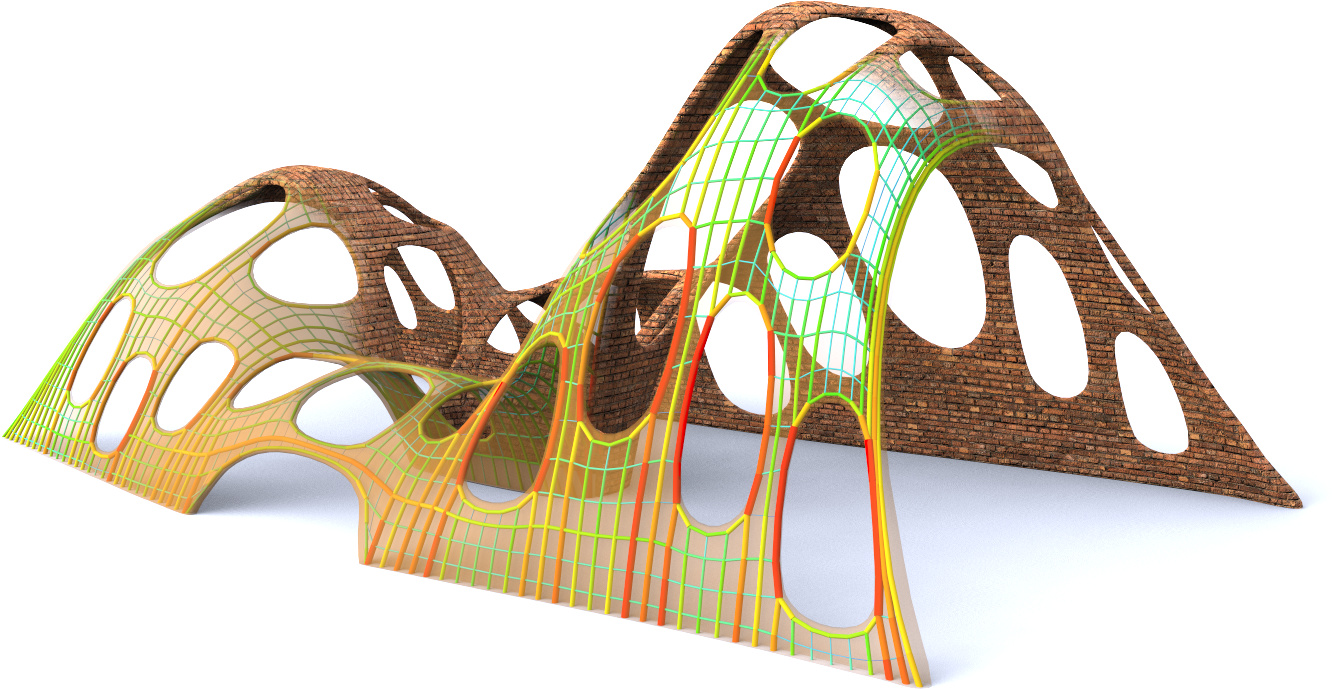
\includegraphics[width=\columnwidth]{arch-fig/cheesevault78.jpg}
	\caption{Surfaces with irregularly placed holes almost
never stand by themselves when built from bricks; for those that do,
stability is not obvious by inspection. The surface shown is produced by
finding the nearest self\dash supporting shape from a given freeform
geometry. The image also illustrates
the fictitious thrust network used in our algorithm,
with edges' cross-section and coloring visualizing the magnitude of
forces (warmer colors represent higher stresses.)}
	\label{fig:cheese}
\end{figure}
}



\paragraph{Contributions.}


$\bullet$ We present an optimization algorithm, based on the theory of
thrust networks and Airy potentials, for efficiently finding a
self\dash supporting surface near a given arbitrary reference surface
\secref{sec:opt}, and build a tool for interactive design of
self\dash supporting surfaces based on this algorithm \secref{sec:design}.
Freeform masonry is based on such surfaces.

$\bullet$ The discrete ``stress Laplacian''
derived from a thrust network with compressive
forces is a so\dash called perfect one \secref{sec:thrustnetworks}.
We use it to argue why our discretizations are 
faithful to the continuous case.

$\bullet$ We connect the physics of self\dash supporting surfaces with
the geometry of isotropic 3\dash space, and express the
equations governing self\dash supporting surfaces in terms of curvatures
\secref{sec:smooth} and \secref{sec:discrete}.
Likewise we establish a connection between the stress Laplacian and
mean curvatures of polyhedral surfaces. This theoretical part of the
paper is a contribution to Discrete Differential Geometry.


$\bullet$ We use the geometric knowledge we have gathered to 
find particularly nice families of self\dash supporting surfaces,
especially planar quadrilateral representations of thrust networks
\secref{sec:special}. This leads to steel\slash glass structures
with low bending and torsion moments.



\paragraph{Related Work.}

Unsupported masonry has been an active topic of research in the
engineering community. The foundations for the modern approach were laid
by Jacques Heyman \shortcite{Heyman66} and are available as the textbook
\cite{Heyman95}. The theory of reciprocal force diagrams in the planar
case was studied by J.~Maxwell;
a unifying view on polyhedral surfaces, compressive
forces and corresponding ``convex'' force diagrams is presented by
\cite{Ash1988}. F.~Fraternali \shortcite{Fraternali2002a,Fraternali2010} established a connection between the continuous
theory of stresses in membranes and the discrete theory of forces in
thrust networks, by interpreting the latter as a non-conforming
finite element discretization of the former.

Several authors have studied the problem of finding discrete compressive
force networks contained within the boundary of masonry structures; previous
work in this area includes \cite{O'Dwyer98} and
\cite{andreu-2007}. Fraternali~\shortcite{Fraternali2010} proposed solving
for the structure's discrete stress surface, and examining its convex hull
to study the structure's stability and susceptibility to cracking. \newtext{This approach works well for analyzing existing structures, where the boundary tractions can be measured and the stress surface is known to be close to convex, but is not an ideal design tool since in such settings the boundary tractions are unknown, and where replacing a non-convex intial stress surface by its convex hull can cause large, uncontrolled global changes to the surface being designed.}
Philippe Block's seminal thesis introduced {\it Thrust
Network Analysis}, which pioneered the use of thrust networks and their
reciprocal diagrams for efficient and practical design of self\dash supporting
masonry structures. By first seeking a reciprocal diagram of the top view, guaranteeing equilibrium
of horizontal forces, then solving for the heights that balance the
vertical loads, Thrust Network Analysis linearizes the form-finding problem.
For a thorough overview of this methodology, see e.g.\ \cite{Block07,block09}.
Recent work by Block and coauthors extends this method in the case where the reciprocal diagram
is not unique; for different choices of reciprocal diagram, the optimal
heights can be found using the method of least squares~\cite{vanmele2011},
and the search for the best such reciprocal diagram can be automated using
a genetic algorithm~\cite{Block2011}.

Other approaches to the design of self-supporting structures
include modeling these structures as damped particle-spring
systems \newtext{(``dynamic relaxation'' methods)}~\cite{Kilian2005,barnes09}, and mirroring the rich tradition in
architecture of designing self-supporting surfaces using \newtext{hanging chain
or membrane models (for instance by Frei Otto, Antoni Gaudi, and Heinz Isler)~\cite{Heyman98,Kotnik12}.} \newtext{Force density methods~\cite{linkwitz71} linearize the form-finding problem by solving for static equilibrium with respect to position variables, given prescribed prestresses in the form of axial force densities~\cite{grundig00}.} Alternatively, masonry structures can be
represented by networks of rigid blocks~\cite{Livesley92}, whose conditions
on the structural feasibility were incorporated into procedural modeling
of buildings~\cite{Whiting09}.

Algorithmic and mathematical methods relevant to this paper are work on
the geometry of PQ meshes \cite{Liu2006},
discrete curvatures for such meshes \cite{Pottmann2007b,bobenko-2010-ct},
in particular curvatures in isotropic geometry \cite{Pottmann2007}.
Schiftner and Balzer \shortcite{Schiftner2010} discuss approximating a
reference surface by a quad mesh with planar faces, whose layout is guided
by statics properties of that surface.

\section{Self-supporting Surfaces}

This section contains the theoretical basis of the paper. \newtext{We begin in \S\ref{ssec:cont}
and \S\ref{sec:thrustnetworks} with a review of the continuous theory of self-supporting surfaces, and their discretization as thrust networks~\cite{Block07}. This discrete model and its associated equilibrium equations form the groundwork of our optimization algorithm (\S\ref{sec:design}) for designing self-supporting surfaces. In \S\ref{sec:smooth}, \S\ref{sec:discrete}, and \S\ref{sec:convergence} we draw connections
between the theory of self-supporting surfaces, curvature measures in isotropic geometry, and discrete Laplace-Beltrami operators. These insights lead to some observations on existence of convergence of discrete approximations to smooth self-supporting surfaces, and are important for the later discussions of planar quad remeshing and special classes of self-supporting surfaces (\S\ref{sec:special}).}

\subsection{The Continuous Theory}
\label{ssec:cont}

We model masonry as a surface given by a height field $s(x,y)$
defined in some planar domain $\Omega$. \newtext{We assume a vertical
load density $F(x,y)$ over the top view} --- usually $F$ represents the structure's own weight. By
definition this surface is self\dash supporting if and only if there
exists \newtext{a negative semidefinite (compressive) stress tensor $\sigma$ over the surface whose stresses are in equilibrium with the
acting forces. Rewriting the equilibrium equations in plane coordinates $(x,y)$, we have that such a stress tensor exists if and only if there exists a field $M(x,y) = -\sigma g^{-1} \det g$ of
$2\times 2$ symmetric positive semidefinite matrices satisfying}
	\begin{align}
	\Div (M\nabla s) = F, \quad
	\Div M &= 0,
	  \label{eq:conds}
	\end{align}
 \newtext{where $g$ is the induced metric $\left[\begin{smallmatrix}1+z_x^2 & z_xz_y \\ z_xz_y & 1+z_y^2\end{smallmatrix}\right]$ and} the divergence operator $\Div{u(x,y)\choose v(x,y}= u_x + v_y$ is
understood to act on the columns of a matrix (see e.g.\
\cite{Fraternali2010}, \cite{Giaquinta1985}).

The condition $\Div M=0$ says that $M$ is locally the Hessian of a
real\dash valued function $\phi$ (the {\em Airy stress potential}): With
the notation
	\begin{align*}
	M =
	{\textstyle {m_{11} \ m_{12} \choose m_{12} \ m_{22}}}
	\iff	
	\wh M =
	{\textstyle {\hphantom{-}m_{22} \ -m_{12} \choose -m_{12}
		 \ \hphantom{-}m_{11}}}
	\end{align*}
 it is clear that $\Div M=0$ is an integrability condition for $\wh M$, so
locally there is a potential $\phi$ with
	$$\wh M = \Hess\phi, \quad \text{i.e.,}\quad
	M = \wh{\Hess\phi}.$$
 If the domain $\Omega$ is simply connected, this relation holds globally.
Positive semidefiniteness of $M$ (or equivalently of $\wh M$)
characterizes {\em convexity} of the Airy potential $\phi$. The Airy
function enters computations only by way of its derivatives, so global
existence is not an issue.

{\it Remark:} Stresses at boundary points depend on the way the surface is
anchored: A fixed anchor means no condition, but a free boundary with
outer normal vector $\nw$ means $\<M \nabla s, \nw \> = 0$.


\paragraph{Stress Laplacian.} Note that $\Div M =0$ yields $\Div(M\nabla
s)$ $ =$ $ \tr(M\Hess s)$, which we like to call $\Delta_\phi s$. The
operator $\Delta_\phi$ is symmetric. It is elliptic (as a Laplace operator
should be) if and only if $M$ is positive definite, i.e., $\phi$ is
strictly convex. The balance condition \eqref{eq:conds} may be written as
	$
	\Delta_\phi s = F.
	$


\subsection{Discrete Theory: Thrust Networks}
\label{sec:thrustnetworks}

We discretize a self-supporting surface by a mesh $\SS=(V,E,F)$
(see Figure~\ref{fig:reciprocal}). Loads are again vertical,
and following Block~\shortcite{Block07} we discretize them as force densities $F_i$ associated with vertices
$\vw_i$. The load acting on this vertex is then given by $F_iA_i$, where
$A_i$ is an area of influence (using a prime to indicate projection onto
the $xy$ plane, $A_i$ is the area of the Voronoi cell of $\vw_i'$ w.r.t.\
$V'$). We assume that stresses are carried by the edges of the mesh: the
force exerted on the vertex $\vw_i$ by the edge connecting $\vw_i,\vw_j$
is given by
	\begin{align*}
	w_{ij} (\vw_j-\vw_i),
	\quad
	\text{where}\quad
	w_{ij}=w_{ji}\ge 0.
	\end{align*}
 The nonnegativity of the individual weights $w_{ij}$ expresses the
compressive nature of forces. The balance conditions at vertices then read
as follows: With $\vw_i=(x_i,y_i,s_i)$ we have
	\begin{align}
	\sum\nolimits_{j\sim i}
		w_{ij} (x_j - x_i)
	=
	\sum\nolimits_{j\sim i}
		w_{ij} (y_j - y_i) &= 0,
			 \label{eq:deqtop} \\
	\sum\nolimits_{j\sim i}
		w_{ij} (s_j - s_i)
		&= A_i F_i.
			\label{eq:deqz}
	\end{align}
 A mesh equipped with edge weights in this way is a discrete \emph{thrust
network}~\cite{block09}. Invoking the safe theorem, we can state that a masonry structure
is self\dash supporting, if we can find a thrust network with compressive
forces which is entirely contained within the structure.

  \begin{figure}[t]
  \centering
  \begin{overpic}[width=.94\columnwidth]{fig/reciprocal}
	\put(0,33){$\SS$}
	\lput(13,33){$\vw_i$}
	\cput(14,25){\contour{white}{$A_iF_i$}}
	\color{gelb}
	\lput(100,19){$\SS'^*$}
	\color{blau}
	\put(0,9){$\SS'$}
	\color{drot}
	\put(1,0){$w_{ij} \ew_{ij}'$}
	\lput(63,3){$\ew_{ij}^*$}
  \end{overpic}
 \caption{A thrust network $\SS$ with dangling edges indicating external
forces (left). This network together with compressive forces which balance
vertical loads $A_iF_i$ projects onto a planar mesh $\SS'$ with
equilibrium compressive forces $w_{ij}\ew_{ij}'$ in its edges. Rotating
forces by 90$^\circ$ leads to the reciprocal force diagram $\SS'^*$
(right).}
  \label{fig:reciprocal}
  \end{figure}

\paragraph{Reciprocal Diagram.}

Equations \eqref{eq:deqtop} have a geometric interpretation: with edge
vectors
	\begin{align*}
	\ew'_{ij} = \vw_j'-\vw_i'=(x_j, y_j) - (x_i, y_i),
	\end{align*}
 Equation \eqref{eq:deqtop} asserts that vectors $w_{ij} \ew_{ij}'$ form a
closed cycle. Rotating them by 90 degrees, we see that likewise
	\begin{align*}
	\ew_{ij}^{\prime *} = w_{ij} J \ew_{ij}', \quad \text{with}\quad
	J={\textstyle{0 \ -1 \choose 1 \ \hphantom{-}0}},
	\end{align*}
 form a closed cycle (see Figure \ref{fig:reciprocal}). If the mesh $\SS$
is simply connected, there exists an entire {\em reciprocal diagram}
$\SS^{\prime *}$ which is a combinatorial dual of $\SS$, and which has
edge vectors $\ew_{ij}'^*$~\cite{Block07}. Its vertices are denoted by $\vw_i^{\prime
*}$.

{\it Remark:} If $\SS'$ is a Delaunay triangulation, then the
corresponding Voronoi diagram is an example of a reciprocal diagram.

\paragraph{Polyhedral Stress Potential.}

We can go further and construct a convex polyhedral ``Airy stress
potential'' surface $\Phi$ with vertices $\ww_i=(x_i,y_i,\phi_i)$
combinatorially equivalent to $\SS$ by requiring that a primal face of
$\Phi$ lies in the plane $z=\alpha x + \beta y + \gamma$ if and only if
$(\alpha,\beta)$ is the corresponding dual vertex of $\SS'^*$ (see
Figure~\ref{fig:polarity}). Obviously this condition determines $\Phi$ up
to vertical translation. For existence see \cite{Ash1988}. The inverse
procedure constructs a reciprocal diagram from $\Phi$. This procedure
works also if forces are not compressive: we can construct an Airy mesh
$\Phi$ which has planar faces, but it will no longer be a convex
polyhedron.

The vertices of $\Phi$ can be interpolated by a piecewise\dash linear
function $\phi(x,y)$. It is easy to see that the derivative of $\phi(x,y)$
jumps by the amount $\|\ew_{ij}'^*\| = w_{ij}\|\ew_{ij}'\|$ when crossing
over the edge $\ew'_{ij}$ at right angle, with unit speed. This identifies
$\Phi$ as the Airy polyhedron introduced by \cite{Fraternali2002a} as a
finite element discretization of the continuous Airy function (see also
\cite{Fraternali2010}).

If the mesh is not simply connected, the reciprocal diagram and the Airy
polyhedron exist only locally. Our computations do not require global existence.

  \begin{figure}[t]
 \centerline{\vphantom{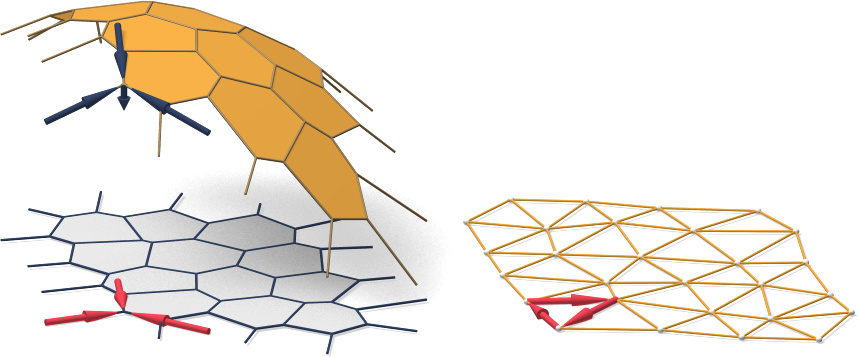
\includegraphics[width=.94\columnwidth]
		{fig/reciprocal}}\relax
  \begin{overpic}[width=.85\columnwidth]{fig/beide}
	\lput(49,33){$\ww_k^*$}
	\lput(49,15){$\vw_k^{*\prime}$}
	\color{gelb}
	\put(86,10){$\SS'^*=\Phi^{*\prime}$}
	\put(83,30){$\Phi^*$}
	\color{blau}
	\cput(24,35){$\Phi$}
	\put(0,0){$\Phi'=\SS'$}
	\cput(4,31){$f_k$}
  \end{overpic}}
 \caption{Airy stress potential $\Phi$ and its polar dual $\Phi^*$. $\Phi$
projects onto the same planar mesh as $\SS$ does, while $\Phi^*$ projects
onto the reciprocal force diagram.  A primal face $f_k$ lies in the plane
$z=\alpha x + \beta y + \gamma$ $\iff$ the corresponding dual vertex is
$\ww_k^*=(\alpha,\beta,-\gamma)$.}
  \label{fig:polarity}
  \end{figure}


\paragraph{Polarity.}

Polarity with respect to the {\em Maxwell paraboloid} $z={1\over 2}
(x^2+y^2)$ maps the plane $z=\alpha x + \beta y + \gamma$ to the point
$(\alpha,\beta,-\gamma)$. Thus, applying polarity to $\Phi$ and projecting
the result $\Phi^*$ into the $xy$ plane reconstructs the reciprocal
diagram $\Phi^{*\prime}=\SS^{\prime *}$ (see Fig.~\ref{fig:polarity}).

\paragraph{Discrete Stress Laplacian.}

The weights $w_{ij}$ may be used to define a graph Laplacian $\Delta_\phi$
which on vertex\dash based functions acts as
	\begin{align*}
	\Delta_{\phi} s(\vw_i)=\sum\nolimits_{j\sim i} w_{ij}(s_j-s_i).
	\end{align*}
 This operator is a perfect discrete Laplacian in the sense of
\cite{wardetzky07}, since it is symmetric by construction, Equation
\eqref{eq:deqtop} implies linear precision for the planar ``top view
mesh'' $\SS'$ (i.e., $\Delta_\phi f=0$ if $f$ is a linear function), and
$w_{ij}\ge 0$ ensures semidefiniteness and a maximum principle for
$\Delta_\phi$\dash harmonic functions. Equation \eqref{eq:deqz} can be
written as $\Delta_\phi s = AF$.

Note that $\Delta_\phi$ is well defined even when the underlying meshes
are not simply connected.

\subsection{Surfaces in Isotropic Geometry} \label{sec:smooth}

It is worthwhile to reconsider the basics of self\dash supporting surfaces
in the language of dual\dash isotropic geometry, which takes place in
$\R^3$ with the $z$ axis as a distinguished vertical direction. The basic
elements of this geometry are planes, having equation $z=f(x,y) = \alpha
x+\beta y+\gamma$. The gradient vector $\nabla f = (\alpha,\beta)$
determines the plane up to translation. A plane tangent to the graph of
the function $s(x,y)$ has gradient vector $\nabla s$.

There is the notion of {\em parallel points}:
	$
	(x,y,z) \parallel (x',y',z') \iff
	x=x',\ y=y'
	.$

{\it Remark:} The Maxwell paraboloid is considered the unit sphere of isotropic
geometry, and the geometric quantities considered above are assigned
specific meanings: The forces $\|\ew_{ij}^*\|=w_{ij}\|\ew_{ij}\|$
are dihedral angles of the Airy polyhedron $\Phi$, and also ``lengths'' of
edges of $\Phi^*$. We do not use this terminology in the sequel.

\paragraph{Curvatures.}

Generally speaking, in the differential geometry of surfaces one considers
the {\em Gauss map} $\sigma$ from a surface $S$ to a convex unit sphere
$\Phi$ by requiring that corresponding points have parallel tangent
planes.  Subsequently mean curvature $H^\rel$ and Gaussian curvature
$K^\rel$ {\em relative to $\Phi$} are computed from the derivative
$d\sigma$. Classically $\Phi$ is the ordinary unit sphere $x^2+y^2+z^2=1$,
so that $\sigma$ maps each point to its unit normal vector.



In our setting, parallelity is a property of {\em points} rather than
planes, and the Gauss map $\sigma$ goes the other way, mapping the tangent
planes of the unit sphere $z=\phi(x,y)$ to the corresponding tangent plane
of the surface $z=s(x,y)$. If we know which point a plane is attached to,
then the Gauss map is determined by the plane's gradient. So we simply write
	\begin{align*}
	\nabla \phi\overset\sigma\longmapsto\nabla s.
	\end{align*}
 By moving along a curve $\uw(t)=(x(t),y(t))$ in the parameter domain we
get the first variation of tangent planes:
	$
	{d\over dt}\nabla \phi|_{\uw(t)} =
	(\Hess\phi)\dot\uw
	$.
 This yields the derivative
	$	
	(\Hess\phi)\dot\uw \overset{d\sigma}\longmapsto
	(\Hess s)\dot\uw $,
 for all $\dot\uw$, and the matrix of $d\sigma$ is found as
$(\Hess\phi)^{-1}(\Hess s)$.  By definition, curvatures of the surface $s$
{\em relative} to $\phi$ are found as
	\begin{align*}
		K_s^\rel
	& = \textstyle
		\det(d\sigma) =
		{\det\Hess s \over \det\Hess\phi} ,
	\\
		H_s^\rel
	&= \textstyle
		{1\over 2}\tr(d\sigma)
		= {1\over 2}\tr \left({M\over\det\Hess\phi} \Hess s\right)
		=  {\Delta_\phi s \over 2\det\Hess\phi}.
	\end{align*}
 The Maxwell paraboloid $\phi_0(x,y)={1\over 2}(x^2+y^2)$ is the canonical
unit sphere of isotropic geometry, with Hessian $E_2$. Curvatures
relative to $\phi_0$ are not called ``relative'' and are denoted by the
symbols $H,K$ instead of $H^\rel,K^\rel$. The observation
	\begin{align*}
	\Delta_\phi \phi
	= \tr(M \Hess \phi)
	= \tr(\wh{\Hess\phi}\Hess\phi)
	= 2\det\Hess\phi
	\end{align*}
 together with the formulas above implies
	\begin{align*}
		K_s  = \det \Hess s,
	\
		K_\phi = \det \Hess \phi
		%H_s = {\Delta s \over 2},
		%K_s^\rel = {K_s\over K_\phi}
	\implies
		H_s^\rel =  {\Delta_\phi s \over 2 K_\phi}
			= {\Delta_\phi s\over \Delta_\phi \phi}.
	\end{align*}

\paragraph{Relation to Self-supporting Surfaces.}

Summarizing the formulas above,
we rewrite the balance condition \eqref{eq:conds} as
	\begin{equation}
	2 K_\phi H_s^\rel  = \Delta_\phi s = F.
	\label{equigeo}
	\end{equation}
 Let us draw some conclusions:

\begin{itemize}\itemsep-\parsep

\item Since $H^\rel_\phi=1$ we see that the load $F_\phi=2K_\phi$ is
admissible for the stress surface $\phi(x,y)$, which is hereby shown as
self\dash supporting. The quotient of loads yields
	$
	 H_s^\rel = F/F_\phi.
	$

\item If the stress surface coincides with the Maxwell paraboloid, then
{\em constant loads characterize constant mean curvature surfaces},
because we get $K_\phi=1$ and $H_s=F/2$.

\item If $s_1,s_2$ have the same stress potential $\phi$, then
$H^\rel_{s_1-s_2}=H^\rel_{s_1}-H^\rel_{s_2}=0$, so $s_1-s_2$ is a
(relative) minimal surface.

\end{itemize}



\subsection{Meshes in Isotropic Geometry} \label{sec:discrete}

A general theory of curvatures of polyhedral surfaces with respect to a
polyhedral unit sphere was proposed by
\cite{Pottmann2007b,bobenko-2010-ct}, and its dual complement in isotropic
geometry was elaborated on in \cite{Pottmann2007}. As illustrated by
Figure~\ref{fig:christoffel}, the mean curvature of a self\dash supporting
surface $\SS$ {\em relative} to its discrete Airy stress potential is
associated with the vertices of $\SS$. It is computed from areas and mixed
areas of faces in the polar polyhedra $\SS^*$ and $\Phi^*$:
	\begin{align*}
	H^\rel(\vw_i)
	&= {A_i(\SS,\Phi) \over A_i(\Phi,\Phi)},
	\quad\text{where}
	\\
		A_i (\SS,\Phi)
	&=
		\frac{1}{4}
		\sum_{k:f_k\in \text{1-ring}(\vw_i)}
		\det(\vw'^*_k, \ww'^*_{k+1})
		+ \det(\ww'^*_k, \vw'^*_{k+1}).
	\end{align*}
 The prime denotes the projection into the $xy$ plane, and summation is
over those dual vertices which are adjacent to $\vw_i$.
Replacing $\vw_k^*$ by $\ww_k^*$ yields
	$
		A_i (\Phi,\Phi)
	=
	\frac{1}{2}
		\sum
		\det(\ww'^*_k, \ww'^*_{k+1}).
	$

\begin{figure}[h]
 \centering
 \begin{overpic}[width=.8\columnwidth]{fig/christoffel}
	\put(17,12){$\vw_i$}
	\put(0,8){$\SS$}
	\put(0,30){$\Phi$}
	\color{blau}
	\lput(52,18){$\ww_0^*$}
	\lput(65,22){$\vw_0^*$}
	\lput(60,0){$\ww_1^*$}
	\lput(58,32){$\vw_1^*$}
	\put(91,8){$\ww_2^*$}
	\put(82,37){$\vw_2^*$}
	\put(82,21){$\ww_3^*$}
	\put(89,26){$\vw_3^*$}
	\color{gelb}
	\cput(8,37){$f_0^\Phi$}
	\cput(8,18){$f_0^\SS$}
	\cput(13,27){$f_1^\Phi$}
	\cput(13,9){$f_1^\SS$}
	\cput(29,32){$f_2^\Phi$}
	\cput(29,12){$f_2^\SS$}
	\cput(22,42){$f_3^\Phi$}
	\cput(22,22){$f_3^\SS$}
	\cput(70,37){$\SS^*$}
	\cput(80,0){$\Phi^*$}
 \end{overpic}
 \caption{Mean curvature of a vertex $\vw_i$ of $\SS$: Corresponding edges
of the polar duals $\SS^*$, $\Phi^*$ are parallel, and mean curvature
according to \protect\cite{Pottmann2007b} is computed from the vertices
polar to faces adjacent to $\vw_i$. For valence 4 vertices the case of
zero mean curvature shown here is characterized by parallelity of non\dash
corresponding diagonals of corresponding quads in $\SS^*,\Phi^*$.}
 \label{fig:christoffel}
 \end{figure}



 \begin{figure*}[t]
	\centering
	%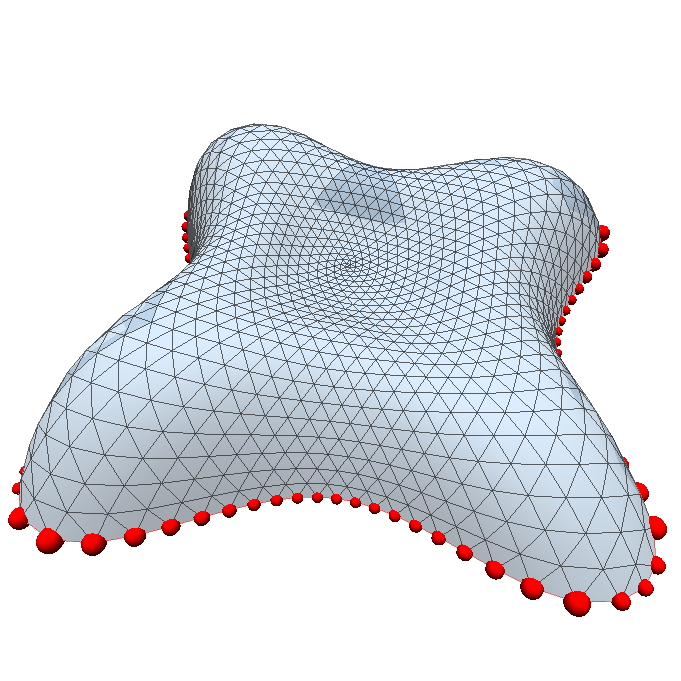
\includegraphics[width=0.24\textwidth]{fig/lilium.png}
	%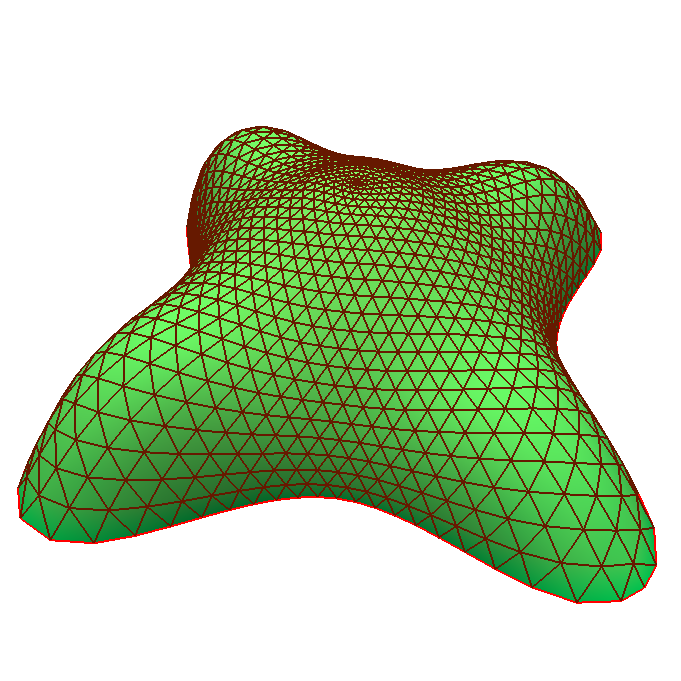
\includegraphics[width=0.24\textwidth]{fig/lilium-n.png}
	%\hfill
	%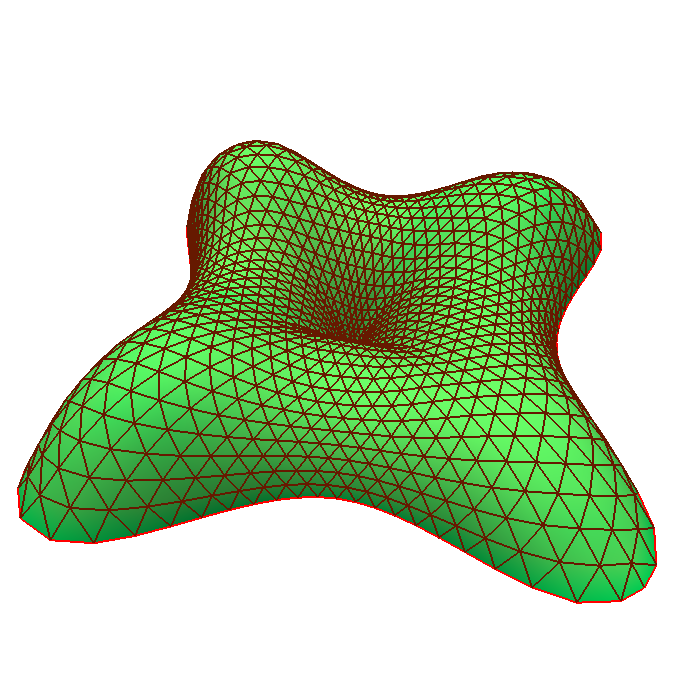
\includegraphics[width=0.24\textwidth]{fig/lilium-pillar-n.png}
	%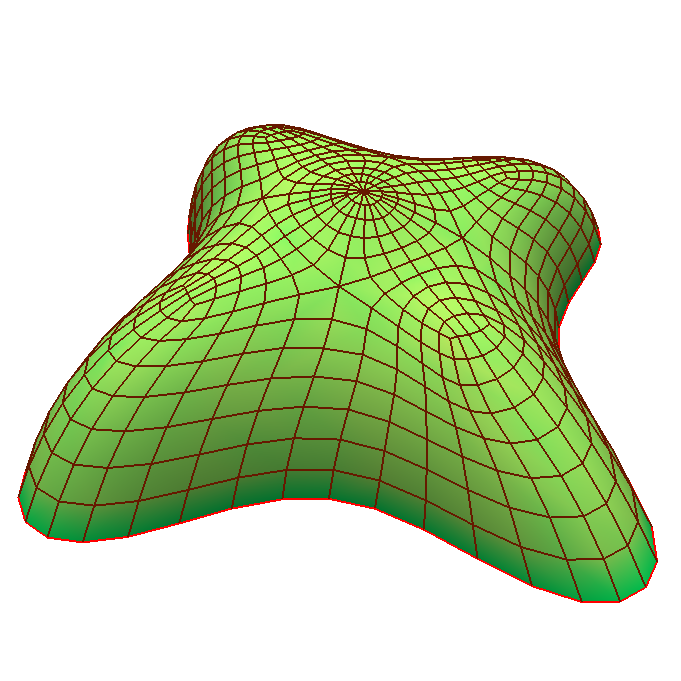
\includegraphics[width=0.24\textwidth]{fig/lilium-pq-n.png}
 \centerline{\begin{overpic}[width=.25\textwidth]{fig/lilium0.jpg}
		\cput(40.05,50){\contour{white}{$\downarrow$}}
		\cput(40,56){\contour{white}{$|$}}
		\cput(40,62){\contour{white}{$|$}}
		\cput(40.05,50){$\downarrow$}
		\cput(40,56){$|$}
		\cput(40,62){$|$}
		\cput(40,72){\small impossible feature}
		\put(0,0){(a)}
	\end{overpic}\hfill
	\begin{overpic}[width=.25\textwidth]{fig/lilium-n.jpg}
		\put(0,0){(b)}
		\color{gelb}
		\put(20,64){$\SS$}
	\end{overpic}\hfill
	\begin{overpic}[width=.25\textwidth]{fig/lilium-nstress.jpg}
		\put(0,0){(c)}
		\color{blau}
		\put(25,60){$\Phi$}
		\lput(45,0){$\SS'^*=\Phi'^*$}
	\end{overpic}\hfill
	\begin{overpic}[width=0.25\textwidth]{fig/lilium-pillar-n2.jpg}
		\put(0,0){(d) \small (view from below)}
	\end{overpic}}
 \caption{The top of the Lilium Tower (a) cannot stand as a masonry
structure, because its central part is concave. Our algorithm finds a
nearby self-supporting mesh (b) without this impossible feature. (c) shows
the corresponding Airy mesh $\Phi$ and reciprocal force diagram $\SS'^*$.
(d) The user can edit the original surface, such as by specifying that the
center of the surface is supported by a vertical pillar, and the
self-supporting network adjusts accordingly.}
 \label{fig:Lilium}
 \end{figure*}



\proclaim Proposition.
 If $\Phi$ is the Airy surface of a thrust network $\SS$, then the mean
curvature of $\SS$ relative to $\Phi$ is computable as
	\begin{equation}
	\label{eq:Hrel}
		H^\rel(\vw_i)
	=
		{\sum_{j\sim i} w_{ij} (s_j-s_i)
		\over \sum_{j\sim i} w_{ij} (\phi_j-\phi_i) }
	=
		{\Delta_\phi s\over \Delta_\phi \phi}\Big|_{\vw_i}.
	\end{equation}

\begin{proof} It is sufficient to show
	$
	2A_i(\SS,\Phi)
	= \sum_{j\sim i} w_{ij} (s_j-s_i).
	$

 For that, consider edges $\ew'_1,\dots,\ew'_n$ emanating from $\vw_i'$.
The dual cycles in $\Phi^{*\prime}$ and $\SS^{*\prime}$ without loss of
generality are given by vertices $(\vw^{*\prime}_1,\dots,\vw^{*\prime}_n)$
and $(\ww^{*\prime}_1,\dots,\ww^{*\prime}_n)$, respectively. The latter
has edges $\ww'^*_{j+1}-\ww'^*_j = w_{ij} J\ew'_j$ (indices modulo $n$).

Without loss of generality $\vw_i=0$, so the vertex $\vw'^*_j$ by
construction equals the gradient of the linear function $\xw\mapsto
\<\vw'^*_j,\xw\>$ defined by the properties $\ew'_{j-1}\mapsto
s_{j-1}-s_i$, $\ew'_j\mapsto s_j-s_i$. Corresponding edge vectors
$\vw'^*_{j+1}-\vw'^*_j$ and $\ww'^*_{j+1}-\ww'^*_j$ are parallel, because
$\<\vw'_{j+1}-\vw'_j,\ew'_j\>=(s_j-s_i)-(s_j-s_i)=0$. Expand
$2A_i(\SS,\Phi)$:
	\begin{align*}
	& \mathrel{\hphantom{=}} \textstyle
		{1\over 2}\sum
		\det(\ww'^*_j, \vw'_{j+1}) + \det(\vw'_j, \ww'^*_{j+1})
	\\
	&=\textstyle
		{1\over 2}\sum
		\det(\ww'^*_j-\ww'^*_{j+1}, \vw'_{j+1})
		+ \det(\vw'_j, \ww'^*_{j+1}-\ww'^*_j)
		\\
	&=\textstyle
		{1\over 2}\sum
		\det( - w_{ij} J\ew'_j, \vw'_{j+1})
	 	+ \det(\vw'_j,w_{ij} J\ew'_j)
	\\
	&= \textstyle
		\sum \det( \vw'_j, w_{ij} J\ew'_j)
	=	 \sum	w_{ij} \< \vw'_j, \ew'_j\>
	= 	 \sum  w_{ij} (s_j-s_i).
	\end{align*}
 Here we have used $\det(\aw,J\bw)=\<\aw,\bw\>$.
 \end{proof}


In order to discretize \eqref{equigeo}, we also need a discrete Gaussian
curvature, usually defined as a quotient of areas which
correspond under the Gauss mapping. We define
	\begin{align*}
	K_\Phi(\vw_i) = {A_i(\Phi,\Phi) \over A_i},
	\end{align*}
 where $A_i$ is the Voronoi area of vertex $\vw_i'$ in the projected mesh
$\SS'$ used in \eqref{eq:deqz}.

{\em Remark:} If the faces of the thrust network $\SS$ are not planar,
the simple trick of introducing additional edges with zero forces in them
makes them planar, and the theory is applicable. In the interest of space, we refrain from elaborating further.


\paragraph{Discrete Balance Equation.}

The discrete version of the balance equation \eqref{equigeo} reads as
follows:

\proclaim Theorem.
 A simply-connected mesh $\SS$ with vertices $\vw_i=(x_i,y_i,s_i)$
can be put into static equilibrium with vertical nodal forces $A_iF_i$ if
and only if there exists a combinatorially equivalent mesh $\Phi$ with
planar faces and vertices $(x_i,y_i,\phi_i)$, such that curvatures of
$\SS$ relative to $\Phi$ obey
	\begin{equation}
	2 K_\Phi(\vw_i) H^\rel(\vw_i) = F_i
	\label{eq:deqiso}
	\end{equation}
 at every interior vertex and every free boundary vertex $\vw_i$. $\SS$
can be put into compressive static equilibrium if and only if there exists
a convex such $\Phi$.

\begin{proof} The relation between equilibrium forces $w_{ij}\ew_{ij}$ in
$\SS$ and the polyhedral stress potential $\Phi$ has been discussed above,
and so has the equivalence ``$w_{ij}\ge 0$ $\iff$ $\Phi$ convex'' (see
e.g.\ \cite{Ash1988} for a survey of this and related results). It remains
to show that Equations \eqref{eq:deqtop} and \eqref{eq:deqiso} are
equivalent. This is the case because the proposition above implies
	$
	2 K(\vw_i) H^\rel(\vw_i) =
	2 \frac{A_i(\Phi,\Phi)}{A_i}
	\frac{A_i(\Phi,\SS)}{A_i(\Phi,\Phi)} =
	{1\over A_i}
	(\sum_{j\sim i} w_{ij} (s_j-s_i))
	= {1\over A_i} A_i F_i.
	$
	\end{proof}

\subsection{Convergence.} \label{sec:convergence}

When considering discrete thrust networks as discretizations of continuous
self\dash supporting surfaces, the following question is important: For a
given smooth surface $s(x,y)$ with stress potential $\phi$, does there
exist a polyhedral surface $\SS$ in equilibrium approximating $s(x,y)$,
whose top view is a given planar mesh $\SS'$? We restrict our attention to
triangle meshes, where planarity of the faces of the discrete stress
surface $\Phi$ is not an issue. Equivalently, we ask:

\begin{itemize}\itemsep-\parsep

\item Does $\SS'$ have a reciprocal diagram whose corresponding Airy
polyhedron $\Phi$ approximates the continuous Airy potential $\phi$? (if
the surfaces involved are not simply connected, these objects are defined
locally).

\item Does $\SS'$ possess a ``perfect'' discrete Laplace\dash Beltrami
operator $\Delta_\phi$ in the sense of Wardetzky et
al.~\shortcite{wardetzky07} whose weights are the edge length scalars of
such a reciprocal diagram?

\end{itemize}

From \cite{wardetzky07} we know that perfect Laplacians exist only on
regular triangulations which are projections of convex polyhedra. On the
other hand, previous sections show how to appropriately re\dash
triangulate: Let $\Phi$ be a triangle mesh convex hull of the vertices
$(x_i,y_i,\phi(x_i,y_i))$, where $(x_i,y_i)$ are vertices of $\SS'$. Then
its polar dual $\Phi^*$ projects onto a reciprocal diagram with positive
edge weights, so $\Delta_\phi$ has positive weights, and the vertices
$(x_i,y_i,s_i)$ of $\SS$ can be found by solving the discrete Poisson
problem $(\Delta_\phi s)_i=A_iF_i$.

We expect, but we don't prove, that the
discrete $\Delta_\phi$
approximates its continuous counterpart for reasonable
sampling (after all it is directly derived from $\phi(x,y)$).
This implies that solving the discrete Poisson equation leads to a mesh
approximating its continuous counterpart $s(x,y)$, and we have
convergence as the sampling density increases.
A rigorous analysis is a  topic for future research.





\section{Thrust Networks from Reference Meshes} \label{sec:opt}

Consider now the problem of taking a given reference mesh, say $\RR$, and
finding a combinatorially equivalent mesh $\SS$ in static equilibrium
approximating $\RR$. The loads on $\SS$ include user-prescribed loads as
well as the dead load caused by the mesh's own weight. Conceptually,
finding $\SS$ amounts to minimizing some formulation of distance between
$\RR$ and $\SS$, subject to constraints \eqref{eq:deqtop},
\eqref{eq:deqz}, and $w_{ij} \geq 0$. For any choice of distance this
minimization will be a nonlinear, non-convex, inequality-constrained
variational problem. Our experience with black-box solvers 
\cite{ipopt} is that
they perform well for surfaces without complex geometry or for
polishing reference meshes close to self-supporting, but fail to converge
in reasonable time for more complicated shapes such as the one of
Fig.~\ref{fig:teaser}, left.
We therefore propose the following specialized, staggered linearization for solving the optimization problem:


\begin{enumerate}\itemsep-\parsep\setcounter{enumi}{-1}

\item Start with an initial guess $\SS = \RR$.

\item \label{step2} Estimate the self\dash load on the vertices of $\SS$,
using their current positions.

\item \label{step3} Fixing $\SS$, locally fit an associated stress surface $\Phi$.

\item \label{step4} Alter positions $\vw_i$ to improve the fit.

\item Repeat from Step~\ref{step2} until convergence.

\end{enumerate}

{\it Remark:} This staggered approach shares several advantages of
solving the full nonlinear problem: a nearby self\dash supporting surface
is found given only a suggested reference shape, without needing to single
one of the many possible top view reciprocal diagrams or needing to
specify boundary tractions -- these are found automatically during
optimization. Although providing an initial top view graph with good
combinatorics remains important, by not fixing the top view our approach
allows the thrust network to slide both vertically and tangentially to the
ground, essential to finding faithful thrust networks for surfaces with
free boundary conditions.

\paragraph{Step~\ref{step2}: Estimating Self-Load.}

The dead load due to the surface's own weight depends not only on the top
view of $\SS$, but also on the surface area of its faces. To avoid adding
nonlinearity to the algorithm, we estimate the load coefficients $F_i$ at
the beginning of each iteration, and assume they remain constant until the
next iteration. We estimate the load $A_iF_i$ associated with each
vertex by calculating its Voronoi surface area on each of its incident faces
(note that this surface area is distinct from $A_i$, the vertex's Voronoi
area on the top view), and then multiplying by a user-specified surface density $\rho$.

\paragraph{Step~\ref{step3}: Fit a Stress Surface.}

In this step, we fix $\SS$ and try to fit a stress surface $\Phi$
subordinate to the top view $\SS'$ of the primal mesh. We do so by
searching for dihedral angles between the faces of $\Phi$ which minimize,
in the least-squares sense, the error in force equilibrium
\eqref{eq:deqiso} and local integrability of $\Phi$. Doing so is
equivalent to minimizing the squared residuals of Equations
\eqref{eq:deqz} and \eqref{eq:deqtop}, with the positions
held fixed. We define the {\em equilibrium energy}
	\begin{align}
	E = \sum\nolimits_i \Big\| \Forcevector -
		\sum\nolimits_{j\sim i} w_{ij} (\vw_j-\vw_i) \Big\|^2,
	\label{eq:eenergy}
	\end{align}
 where $i$ runs through interior and free boundary vertices, and
solve
	\begin{align}
	\min\nolimits_{w_{ij}} E,
	\quad
	\textrm{s.t.}\ \
		0 \leq w_{ij} \leq w_{\max}.
	\label{eq:wbounds}
	\end{align}
 Here $w_{\max}$ is an optional maximum weight we are willing to assign
(to limit the amount of stress in the surface). This convex, sparse,
box-constrained least-squares problem \cite{BCLS} always has a solution.
If the objective is $0$ at this solution, $\SS$ is self-supporting -- we are done. Otherwise, $\SS$
is not self-supporting and its vertices must be moved.

\begin{figure}[t]
	\centerline{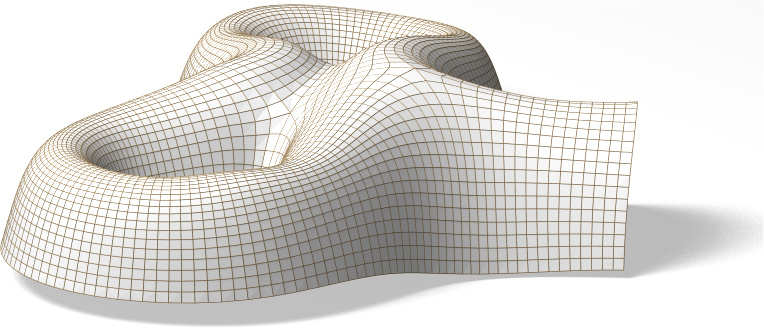
\includegraphics[height=0.11\textwidth]{fig/cas.jpg}\relax
	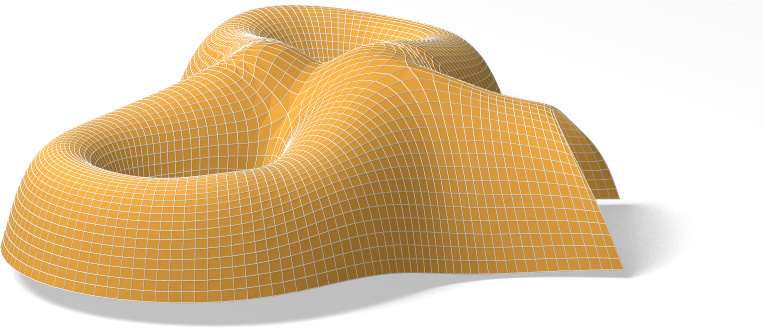
\includegraphics[height=0.11\textwidth]{fig/cas-n.jpg}}
	\caption{A freeform surface
(left) needs adjustments around the entrance arch and between the two
pillars in order to be self-supporting; our algorithm finds the nearby
surface in equilibrium (right) that incorporates these
changes.}\label{fig:cas}
	 \end{figure}


\begin{table}[t]
\begin{tabular}{@{}lccccr@{}}
	%	\textit{Example} &
		 \textit{Fig.}
		& \textit{Vertices}
		& \textit{Edges}
			& \textit{Time} (s)
			& \!\!\!\textit{Iterations} \!\!\!\!
			& \textit{Max.\ Rel.\ Error} \\
	\hline
	%	Top of Lilium Tower &
		 \protect\ref{fig:Lilium}b
		& 1201
		& 3504
			& 21.6
			& 9
			& $4.2 \times 10^{-5}$
	\\ %Top of Lilium Tower (with pillar)  &
		 \protect\ref{fig:Lilium}d
		& 1200
		& 3500
			& 26.5
			& 10
			& $8.5 \times 10^{-5}$
	\\ %Freeform Structure with Two Pillars  &
		 \protect\ref{fig:cas}
		& 1535
		& 2976
			& 17.0
			& 21
			& $2.7\times 10^{-5}$
	\\ %Brick Domes  &
		 \protect\ref{fig:removal}
		& 752
		& 2165
			& 8.0
			& 9
			& $5.8 \times 10^{-5}$
	\\ %Swiss Cheese  &
		 \protect\ref{fig:cheese2}
		& 2358
		& 4302
			& 19.5
			& 9
			& $3.0 \times 10^{-4}$
	\\ %Structural Glass  &
		 \protect\ref{fig:structural}
		& 527
		& 998
			& 5.7
			& 25
			& $2.4\times 10^{-5}$
	\\ \hline
  \end{tabular}
 \def\Tmp{A_iF_i(\raise.4ex\hbox{\tiny
	$\begin{array}{@{}c@{}}0\\[-1ex]0\\[-1ex]1\end{array}$})}
	\caption{Numerical details about our examples.
We show the clock time needed by an Intel Xeon 2.3GHz
desktop PC with 4 GB of RAM to find a self\dash supporting thrust network and
associated stress surface from the example's reference mesh; we also give
the number of outer iterations of the four steps in \secref{sec:opt}. The
maximum relative error is the dimensionless quantity
$\max_i \| \protect\Tmp - \sum\nolimits_{j\sim i} w_{ij}
(\vw_j-\vw_i) \|/A_i F_i$ (the maximum is
taken over interior vertices $\vw_i$).}\label{table:data}

\end{table}

\paragraph{Step~\ref{step4}: Alter Positions.} In the previous step we fit
as best as possible a stress surface $\Phi$ to $\SS$. There are two
possible kinds of error with this fit: the faces around a vertex
(equivalently, the reciprocal diagram) might not close up; and the
resulting stress forces might not be exactly in equilibrium with the
loads. These errors can be decreased by modifying the top view and heights
of $\SS$, respectively. It is possible to simply solve for new vertex
positions that put $\SS$ in static equilibrium, since Equations
\eqref{eq:deqtop} and \eqref{eq:deqz} with $w_{ij}$ fixed form a square
linear system that is typically nonsingular.

While this approach would yield a self-supporting $\SS$, this mesh is
often far from the reference mesh $\RR$, since any local errors in the
stress surface from Step~\ref{step3} amplify into global errors in $\SS$.
We propose instead to look for new positions that decrease the imbalance
in the stresses and loads, while also penalizing drift away from the
reference mesh:
	\begin{align*}
	\min\nolimits_{\vw} E
	+ \alpha \sum\nolimits_i
		\<\nw_i, \vw_i - \vw^0_i \>^2
		+ \beta \big\|\vw - \vw^0_P\big\|^2,
	\end{align*}
 where $\vw^0_i$ is the position of the $i$-th vertex at the start of this
step of the optimization, $\nw_i$ is the starting vertex normal (computed
as the average of the incident face normals), $\vw^0_P$ is the projection
of $\vw^0$ onto the reference mesh, and $\alpha > \beta$ are penalty
coefficients that are decreased proportionally to the decrease in $E$ at every iteration of Steps
\ref{step2}--\ref{step4}. The second term allows $\SS$ to
slide over itself (if doing so improves equilibrium) but penalizes drift
in the normal direction. The third term, weaker than the second,
regularizes the optimization by preventing large drift away from the
reference surface or excessive tangential sliding.

\paragraph{Implementation Details.}

Solving the weighted least\dash squares problem of Step~\ref{step4}
amounts to solving a sparse, symmetric linear system. While the {\sc Minres}
algorithm~\cite{paige75} is likely the most robust algorithm for solving
this system, in practice we have observed that the method of conjugate
gradients works well despite the potential ill-conditioning of the
objective matrix.





\paragraph{Limitations.}

This algorithm is not guaranteed to always converge; this fact is not
surprising from the physics of the problem (if the boundary of the
reference mesh encloses too large of a region, $w_{\max}$ is set too low,
and the density of the surface too high, a thrust network in equilibrium
simply does not exist -- the vault is too ambitious and cannot be built to
stand; pillars are needed.)

We can, however, make a few remarks. Only Step~\ref{step2} can 
increase the equilibrium
 energy $E$ of Equation~\eqref{eq:eenergy}.
Step~\ref{step3} always decreases it, and Step~\ref{step4} does as well as $\beta \to 0$. Moreover, as $\alpha
\to 0$ and $\beta \to 0$, Step~\ref{step4} approaches a linear system with
as many equations as unknowns; if this system has full rank, its solution
sets $E=0$. These facts suggest that the algorithm should generally
converge to a thrust network in equilibrium, provided that
Step~\ref{step2} does not increase the loads by too much at every
iteration, and this is indeed what we observe in practice. One case where
this assumption is guaranteed to hold is if the thickness of the surface
is allowed to freely vary, so that it can be chosen so that the surface
has uniform density over the top view.

If the linear system in Step~\ref{step4} is singular and infeasible, the
algorithm can stall at $E > 0$. This failure occurs, for instance, when an
interior vertex has height $z_i$ lower than all of its neighbors, and
Step~\ref{step3} assigns all incident edges to that vertex a weight of
zero: clearly no amount of moving the vertex or its neighbors can bring
the vertex into equilibrium. We avoid such degenerate configurations by
bounding weights slightly away from zero in \eqref{eq:wbounds}, trading
increased robustness for slight smoothing of the resulting surface. Attempting
to optimize meshes that have self-intersecting top views (i.e., aren't height fields),
have too many impossible features, or are insufficiently supported by fixed
boundary points can also result in errors and instability.

\nix{
\begin{figure}[t]
	%\begin{overpic}[width=0.25\textwidth]{fig/build-white.jpg}
	%\begin{overpic}[width=0.25\textwidth]{fig/build-n.jpg}
	%\begin{overpic}[width=0.25\textwidth]{fig/build-edited-white.jpg}
	%\begin{overpic}[width=0.25\textwidth]{fig/build-edited-n.jpg}
	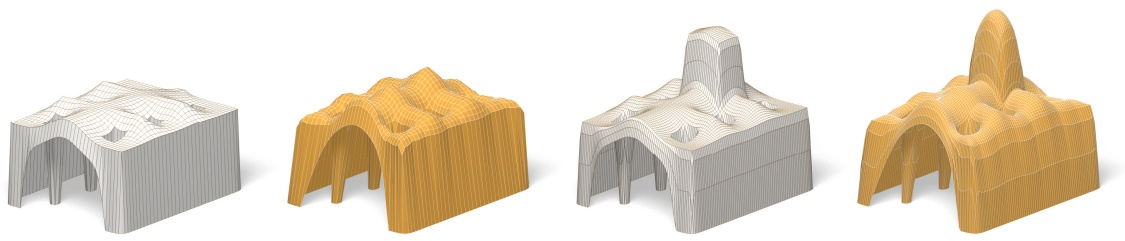
\includegraphics[width=\columnwidth]{fig/edits.jpg}
	\vskip-5em
	(a)\hfill(b)\hfill(c)\hfill(d)\hfill~~
	\vskip3.5em

\caption{The user-designed reference mesh (a) is not self-supporting,
but our algorithm finds a nearby perturbation of the reference surface
(b) that is in equilibrium. As the user makes edits to the
reference surface (c), the thrust network automatically adjusts
(d).} \protect\label{fig:vault}
	\end{figure}
}

 \begin{figure*}[t]
 \centerline{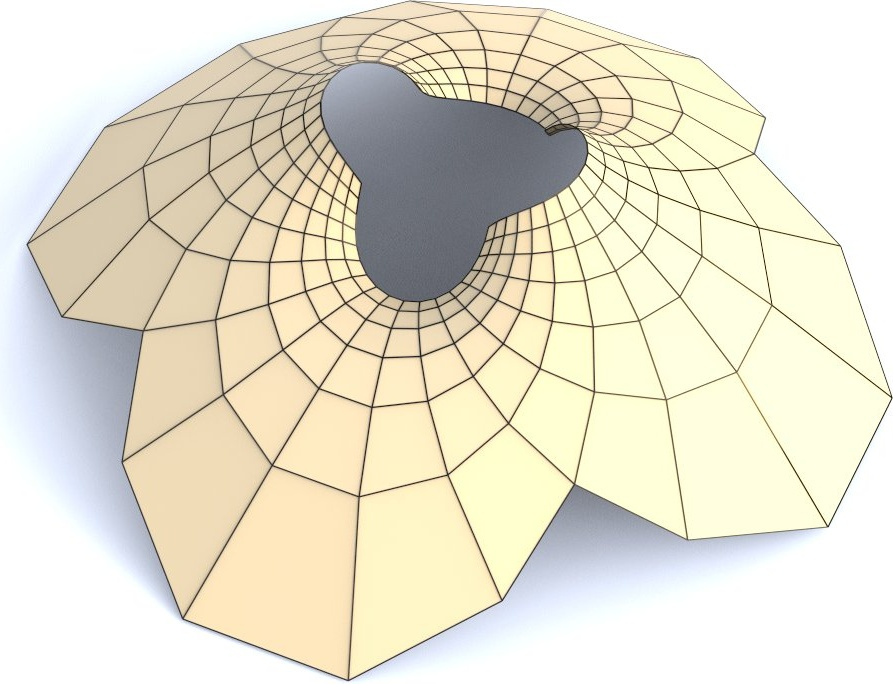
\includegraphics[width=.2\textwidth]{fig/video1}\relax
 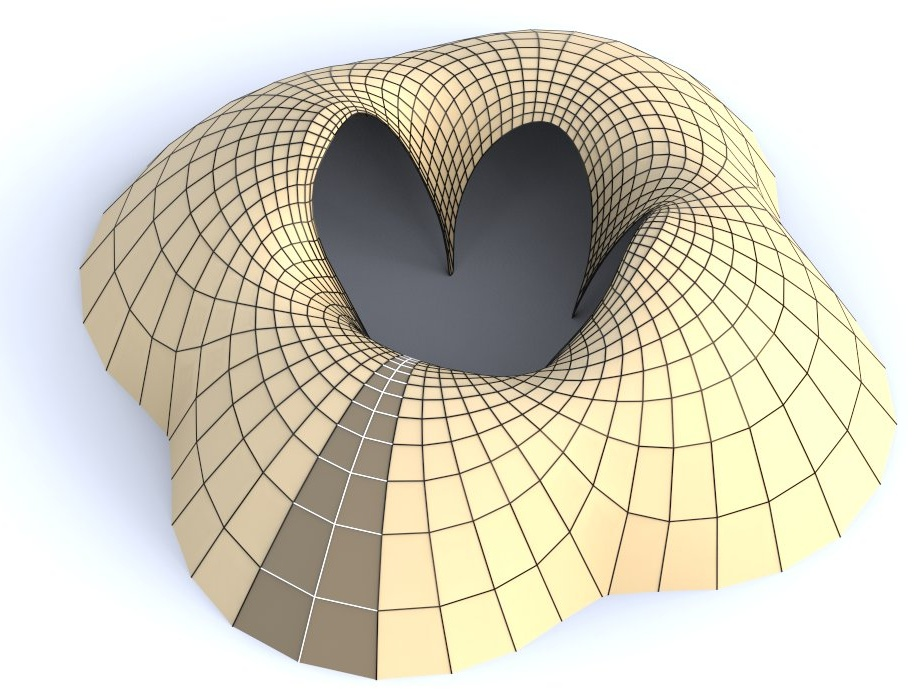
\includegraphics[width=.23\textwidth]{fig/video3}\relax
 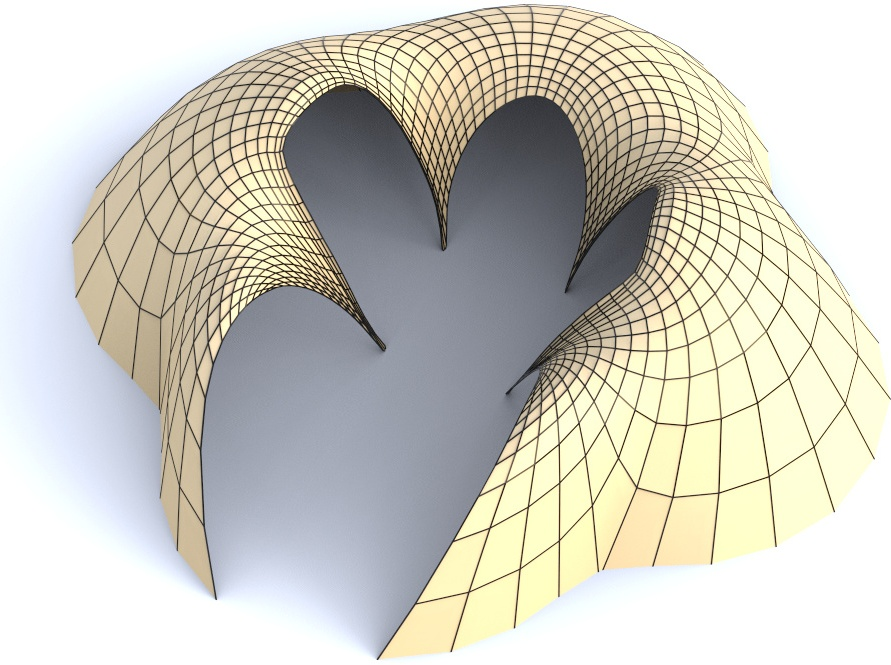
\includegraphics[width=.23\textwidth]{fig/video4}\hfill
 \begin{minipage}[b]{.30\textwidth}
	\caption{Interactive Edits. (a) shows a 
self\dash supporting thrust network --
in fact it is a Koebe mesh as mentioned
in \S\protect\ref{sec:special}.  In (b) boundary conditions
are defined and pillars have been added. Cutting
along the highlighted edge and optimizing for the self\dash supporting
property results in the mesh shown in (c).} \label{fig:edit}
\end{minipage}}

\bigskip

  \newdimen\tmplen\tmplen=0.098\textwidth
 \centerline{\raise.1\tmplen\hbox{\begin{overpic}[width=2.6\tmplen]
		{arch-fig/destruction1.jpg}
		\put(0,10){(a)}
	\end{overpic}}\hfill
	\raise.1\tmplen\hbox{\begin{overpic}[width=2.6\tmplen]
		{arch-fig/destruction2.jpg}
		\put(0,10){(b)}
	\end{overpic}}\hfill
	\begin{overpic}[width=2.6\tmplen]{arch-fig/destruction3.jpg}
		\put(0,10){(c)}
	\end{overpic}\hfill
	\begin{overpic}[width=2.6\tmplen]{arch-fig/destruction4.jpg}
		\put(0,10){(d)}
	\end{overpic}}

\caption{Destruction sequence. We simulate removing small parts of masonry
(their location is shown by a yellow ball) and
the falling off of further pieces which are no longer supported after
removal. For this example, removing a certain small number
of single bricks does not affect stability (a,b). Removal of material at a
certain point (yellow ball in (b))
will cause a greater part of the structure to collapse,
as seen in (c). (d) shows the result after one more removal (all images show
the respective thrust networks, not the reference surface).} \label{fig:removal}
\end{figure*}

%\newtext{This sequence of figures was inspired by images of real-world destruction of masonry structures by the Block Research Group~\protect\cite{catalan}.}


\section{Results}
\label{sec:design}

\paragraph{Interactive Design of Self-Supporting Surfaces.}

The optimization algorithm described in the previous section forms the
basis of an interactive design tool for self-supporting surfaces. Users
manipulate a mesh representing a reference surface, and the computer
searches for a nearby thrust network in equilibrium (see e.g.\
Figure~\ref{fig:edit}). Features of the design tool include:

\begin{itemize}\itemsep-\parsep

\item Handle-based 3D editing of the reference mesh using Laplacian
coordinates~\cite{Lipman2004,Sorkine2003} to extrude vaults, insert
pillars, and apply other deformations to the reference mesh. Handle-based
adjustments of the heights, keeping the top view fixed, and deformation of
the top view, keeping the heights fixed, are also supported. The thrust
network adjusts interactively to fit the deformed positions, giving the
usual visual feedback about the effects of edits on whether or not the
surface can stand.

\item Specification of boundary conditions. Points of contact between the
reference surface and the ground or environment are specified by
``pinning'' vertices of the surface, specifying that the thrust network
must coincide with the reference mesh at this point, and relaxing the
condition that forces must be in equilibrium there.

\item Interactive adjustment of surface density, external loads,
and maximum permissible stress per edge, with visual
feedback of how these parameters affect the fitted thrust network.

\item Upsampling of the thrust network through Catmull\dash Clark
subdivision \nix{\cite{catmull78}}
and polishing of the resulting refined thrust
network using optimization \secref{sec:opt}.

\item Visualization of the stress surface dual to the thrust network
and corresponding reciprocal diagram.

\end{itemize}



\def\sparagraph#1{\par\noindent{\it #1}}


\sparagraph{{\sf\bfseries Examples.} Top of the Lilium Tower:}
Consider the top portion of the steel-glass exterior surface of the Lilium
Tower (being built in Warszaw, see Fig.\
\ref{fig:Lilium}). What is if we had wanted to build this surface
out of masonry instead? This surface contains a concave part with local minimum
in its interior and so cannot possibly be self-supporting without
modification. Given this
surface as a reference mesh, our algorithm constructs a nearby thrust
network in equilibrium without the impossible feature. The user can then
explore how editing the reference mesh -- adding a pillar, for example --
affects the thrust network and its deviation from the reference surface.

\sparagraph{Example: Freeform Structure with Two Pillars.}
Suppose an architect's experience and intuition has permitted the design
of a nearly self\dash supporting freeform surface (Figure \ref{fig:cas}).
Our algorithm reveals those edits needed to make the
structure sound -- principally around the entrance arch, and the area
between the two pillars.

 \begin{figure}[h]
  \centerline{\begin{overpic}[width=0.5\columnwidth]{fig/cheese.jpg}
		\put(0,5){(a)}
	\end{overpic}\relax
	\begin{overpic}[width=0.5\columnwidth]{fig/cheese-n.jpg}
		\put(0,5){(b)}
	\end{overpic}}
  \caption{A mesh with holes (a) requires large deformations
to both the top view and heights to render it self\dash supporting
(b)}\label{fig:cheese2}
  \end{figure}

\begin{figure*}
	\begin{minipage}[b]{\columnwidth}
	\caption{Stability Test. Left: Coloring and cross\dash section
of edges visualize the magnitude of forces in a thrust network which is in
equlibrium with this dome's dead load.
Right: When an additional load is applied, there exists a corresponding
compressive thrust network which is still contained in the masonry hull
of the original dome. This implies stability of the dome under that load.}
\label{fig:load}
	\end{minipage}\hfill
	\begin{overpic}[width=.49\columnwidth]{fig/dome-unloaded.jpg}
		\small
		\cput(30,0){14\,m}
		\put(0,-4){\hbox to .3\columnwidth{\leftarrowfill}}
		\lput(100,-4){\hbox to .3\columnwidth{\rightarrowfill}}
		\put(0,49){shell thickness 0.1\,m, $\rho=2,500$\,kg/m$^3$}
	\end{overpic}\hfill
	\begin{overpic}[width=.49\columnwidth]{fig/dome-loaded.jpg}
		\small
		\put(60,44){11,000\,kg}
	\end{overpic}

\medskip
	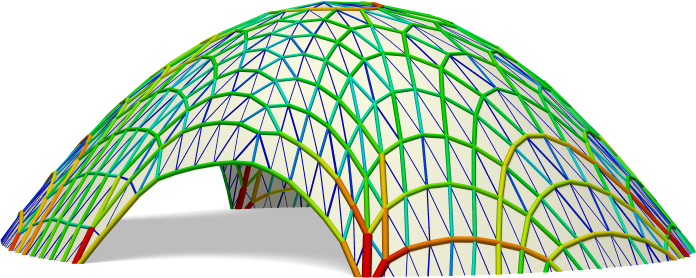
\includegraphics[width=.23\textwidth]{fig/dome2-00.jpg}\hfill
	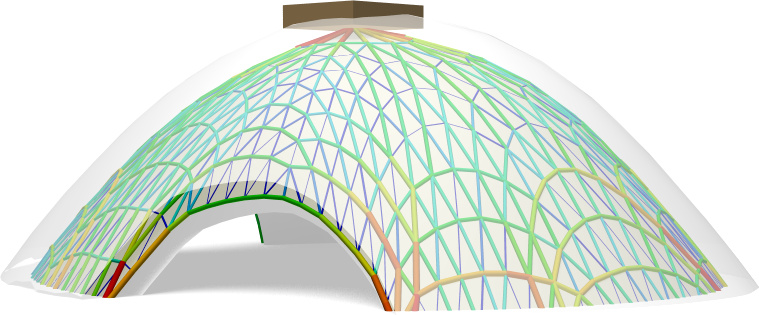
\includegraphics[width=.25\textwidth]{fig/dome2-05.jpg}\hfill
	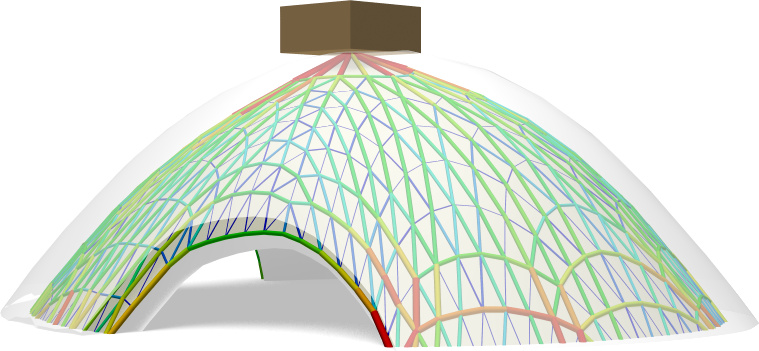
\includegraphics[width=.25\textwidth]{fig/dome2-10.jpg}\hfill
	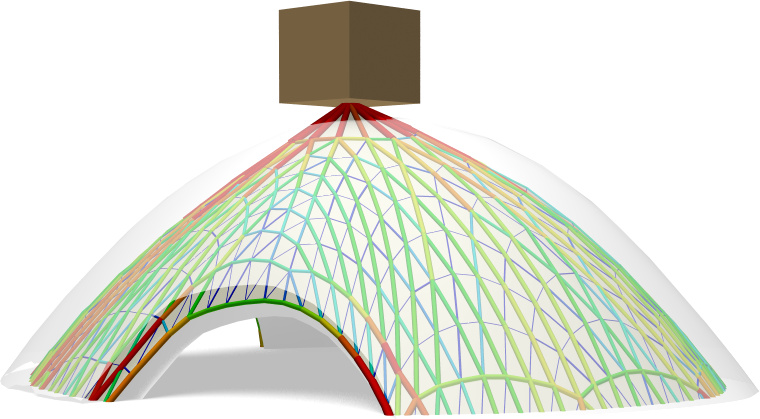
\includegraphics[width=.25\textwidth]{fig/dome2-20.jpg}
	\caption{Stability test similar to Figure~\protect\ref{fig:load},
but with a shell thickness of 1\,m, in order to better visualize the way
the thrust network starts to leave the masonry hull as the load increases.
Additional loads are 0\,kg, 5,000\,kg, 10,000\,kg, and 20,000\,kg, resp., from
left to right.} \label{fig:load2}
%\newtext{These load tests were inspired by real-world experiments performed by the Block Research Group~\protect\cite{catalan,blockfigs}} 


\end{figure*}

\sparagraph{Example: Interactive Editing.}
Figure \ref{fig:edit} shows an example of the design and optimization
workflow. Starting with a mesh, we first add pillars in the center
and clean up the outer boundary (by fixing it to the floor). A subsequent
cut needs a further round of optimization.
This surface is neither convex nor simply connected, and
exhibits a mix of boundary conditions, none of which cause our algorithm
any difficulty; it always finds a self-supporting thrust network near the
designed reference mesh. The user is free to make edits to the
reference mesh, and the thrust network adapts to these edits, providing
the user feedback on whether these designs are physically realizable
{\it [we refer to the accompanying video for interactive building and editing
of freeform self\dash supporting shapes].}

\sparagraph{Example: Destruction Sequence.}
In Figure \ref{fig:removal} we simulate removing parts of masonry and
the falling off of further pieces which are no longer supported after
removal.
This is done by deleting the 1-neighborhood of a vertex
and solving for a new thrust network in compressive equilibrium
close to the original reference surface. We delete those parts of the
network which deviate too much and are no longer contained in the masonry
hull, and iterate.



\sparagraph{Example: Swiss Cheese.}
Cutting holes in a self-supporting surface interrupts force flow lines and
causes dramatic global changes to the surface stresses, often to the point
that the surface is no longer in equilibrium. Whether a given surface with
many such holes can stand is far from obvious. Figure~\ref{fig:cheese2}a
shows such an implausible and unstable surface; our optimization finds a
nearby, equally implausible but stable surface without difficulty 
(Figs.~\ref{fig:teaser}, left and \ref{fig:cheese2}b).

\sparagraph{Example: Stability Test:} See Figures \ref{fig:load},
\ref{fig:load2} for a series of images which visualize the effect of
additional loads on a thrust network.


\sparagraph{Example: Structural Glass}. See Figure \ref{fig:structural} for
details on a self\dash supporting surface which is realized
not as masonry, but as a steel\slash glass construction with glass as
a structural element.


	\begin{figure}[b]
  \centerline{\begin{overpic}[width=0.33\columnwidth]{fig/vault-n.jpg}
	\put(0,0)({(a)}
	\end{overpic}\hfill
  \begin{overpic}[width=0.33\columnwidth]{fig/vault-flat.jpg}
	\put(0,0)({(b)}
	\end{overpic}\hfill
  \begin{overpic}[width=0.33\columnwidth]{fig/vault-pq.jpg}
	\put(0,0)({(c)}
	\end{overpic}}
	\caption{Directly enforcing planarity of the faces of even a very
simple self-supporting quad-mesh vault (a) results in a surface far
removed from the original design (b). Starting instead from a remeshing of
the surface with edges following relative principal curvature directions
yields a self-supporting, PQ mesh far more faithful to the original (c).}
	\label{fig:badpq}
\end{figure}


\section{Special Self-Supporting Surfaces} \label{sec:special}

\paragraph{PQ Meshes.}

Meshes with {\em planar} faces are of particular interest in architecture,
so in this section we discuss how to remesh a given thrust network in
equilibrium such that it becomes a quad mesh with planar faces (again in
equilibrium). If this mesh is realized as a steel\dash glass construction,
it is self\dash supporting in its beams alone, with no forces exerted on
the glass (this is the usual manner of using glass). The beams constitute
a self\dash supporting structure which is in perfect force equilibrium
(without moments in the nodes) if only the deadload is applied.



\begin{figure*}[t]
	%\begin{overpic}[width=.63\textwidth]{fig/lilium_pq3.jpg}
 \begin{minipage}[b]{.27\textwidth}
	\caption{Planar quad remeshing of the surface of
Fig.~\protect\ref{fig:Lilium}. (a) Relative principal directions,
found from eigenvectors of $(\Hess\phi)^{-1}\Hess s$. (b) Quad mesh
guided by principal directions is almost planar and almost self\dash
supporting. (c) Small changes achieve both properties.}
 \label{fig:lilium:pq}\end{minipage}\hfill
	\raise0.02\textwidth\hbox{\begin{overpic}
		[width=.23\textwidth]{fig/lilium-vf.jpg}
		\put(0,0){(a)}
	\end{overpic}}\hfill
	\raise0.02\textwidth\hbox{\begin{overpic}
		[width=.23\textwidth]{fig/lilium-pq.jpg}
		\put(0,0){(b)}
	\end{overpic}}\hfill
	\raise0.02\textwidth\hbox{\begin{overpic}
		[width=.22\textwidth]{arch-fig/lilium-pq-93.jpg}
		\put(0,0){(c)}
	\end{overpic}}

	\begin{minipage}[b]{.27\textwidth}
	\caption{Planar quad remeshing of the surface of
Figure~\protect\ref{fig:cas}. Left: Relative principal directions. Right: The
result of optimization is a self\dash supporting PQ mesh, which guides a
moment\dash free steel\slash glass construction (interior view, see also
Fig.~\protect\ref{fig:teaser}).}
	\label{fig:cas:pq}
	\end{minipage}\hfill
	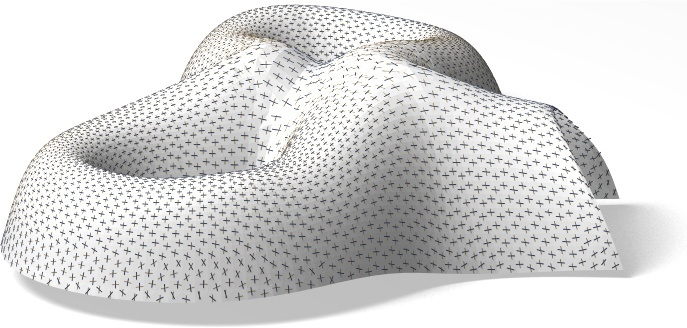
\includegraphics[height=0.17\textwidth]{fig/cas-vf.jpg}\hfill
	%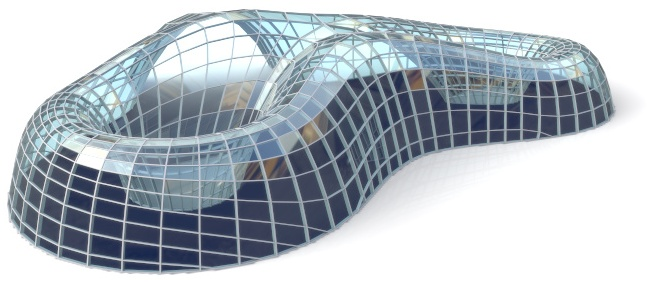
\includegraphics[height=0.15\textwidth]{arch-fig/1roo62.jpg}
	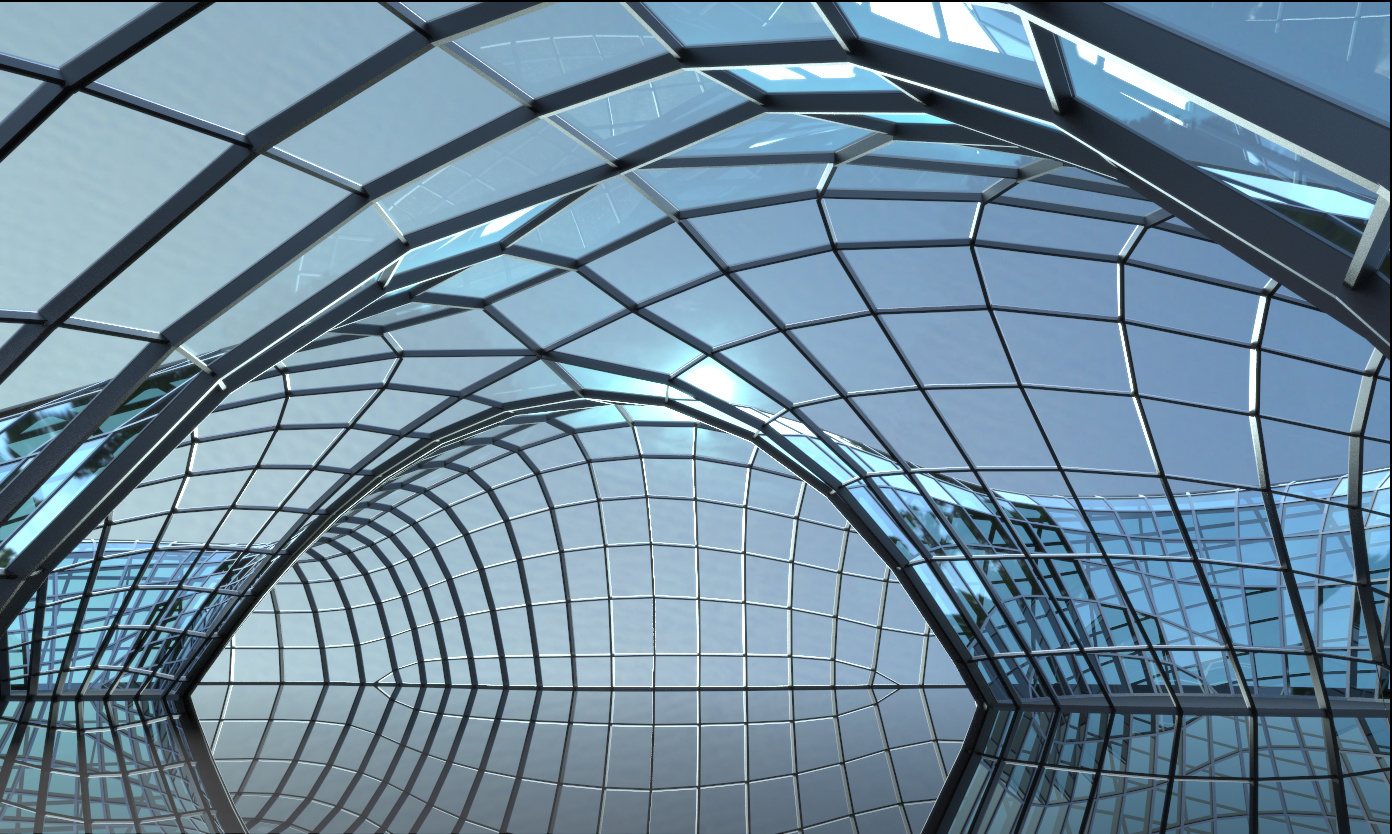
\includegraphics[height=0.15\textwidth]{arch-fig/1roo58.jpg}
  \end{figure*}

Taking an arbitrary non-planar
quad mesh and attempting naive, simultaneous enforcement of planarity and
static equilibrium -- either by staggering a planarity optimization step every outer
iteration, or adding a planarity penalty term to the position update -- does not
yield good results, as shown in Figure~\ref{fig:badpq}. Indeed, as we will see later
in this section, such a planar perturbation of a thrust network is not expected to
generally exist.

Consider a planar quad mesh $\SS$ with vertices
$\vw_{ij}=(x_{ij},y_{ij},s_{ij})$ which approximates a given continuous
surface $s(x,y)$. It is known that $\SS$ must approximately follow a network
of conjugate curves in the surface (see e.g.\ \cite{Liu2006}). We can derive
this condition in an elementary way as follows: Using a Taylor expansion, we
compute the volume of the convex hull of the quadrilateral $\vw_{ij}$,
$\vw_{i+1,j}$, $\vw_{i+1,j+1}$, $\vw_{i,j+1}$, assuming the vertices lie
exactly on the surface $s(x,y)$. This results in
	\begin{align*}
	&\textstyle
	\text{vol} =
	{1\over 6}\det(\aw_1,\aw_2) \cdot
		\left((\aw_1)^T\,\Hess s\,\aw_2 \right)+ \cdots,
	\\
	\text{where}\
	& \textstyle
	\aw_1={x_{i+1,j}-x_{ij}\choose y_{i+1,j}-y_{ij}},\quad
	\aw_2={x_{i,j+1}-x_{ij}\choose y_{i,j+1}-y_{ij}},
	\end{align*}
 and the dots indicate higher order terms. We see that planarity requires
$(\aw_1)^T\,\Hess s\,\aw_2=0$. In addition to the mesh $\SS$ approximating
the surface $s(x,y)$, the corresponding polyhedral Airy surface $\Phi$
must approximate $\phi(x,y)$; thus we get the conditions
	\begin{align*}
	(\aw_1)^T\,\Hess s\,\,\aw_2=
	(\aw_1)^T\,\Hess \phi\,\,\aw_2= 0.
	\end{align*}
 $\aw_1,\aw_2$ are therefore eigenvectors of $(\Hess\phi)^{-1}\Hess s$. In
view of \S\ref{sec:smooth}, $\aw_1,\aw_2$ indicate the principal
directions of the surface $s(x,y)$ relative to $\phi(x,y)$.



In the discrete case, where $s,\phi$ are not given as continuous surfaces,
but are represented by a mesh in equilibrium and its Airy mesh, we use the
techniques of Schiftner~\shortcite{Schiftner2007} and Cohen\dash Steiner
and Morvan \shortcite{Cohen-Steiner2003} to approximate the Hessians
$\Hess s$, $\Hess\phi$, compute principal directions as eigenvectors of
$(\Hess\phi)^{-1}\Hess s$, and subsequently find meshes $\SS,\Phi$
approximating $s,\phi$ which follow those directions. Global optimization
can now polish $\SS,\Phi$ to a valid thrust network with discrete stress
potential, where before it failed: we do so by taking the planarity energy
$\sum_f (2\pi - \theta_f)^2$, where the sum runs over faces and $\theta_f$ is the
sum of the interior angles of face $f$, linearizing it at every iteration, and
adding it to the objective function of the position update (Step \ref{step4}).
Convexity of $\Phi$ ensures that $\SS$ is self\dash supporting.


Note that for each $\Phi$, the relative principal curvature directions give the
\emph{unique} curve network along which a planar quad discretization of a
self\dash supporting surface is possible. Other networks won't work 
(see Figure~\ref{fig:badpq}).
Figures~\ref{fig:lilium:pq} and \ref{fig:cas:pq}
further illustrate the result of applying this procedure to
self-supporting surfaces.




{\em Remark:} When remeshing a given shape by planar quad meshes, we know
that the circular and conical properties require that the mesh follows the
ordinary, Euclidean principal curvature directions \cite{Liu2006}. It is
remarkable that the self\dash supporting property in a similar manner
requires us to follow certain {\em relative} principal directions.
Practictioners' observations regarding the beneficial statics properties
of principal directions can be explained by this analogy, because the
relative principal directions are close to the Euclidean ones, if the
stress distribution is uniform and $\|\nabla s\|$ is small.



\paragraph{Koenigs Meshes.}

Given a self\dash supporting thrust network $\SS$ with stress surface
$\Phi$, we ask the question:
Which vertical perturbation $\SS+\RR$ is self\dash supporting, with the same
loads as $\SS$? As to notation, all involved meshes $\SS,\RR,\Phi$ have the
same top view, and arithmetic operations refer to the respective $z$
coordinates
$s_i,r_i,\phi_i$ of vertices.

The condition of equal loads then is expressed as
$\Delta_\phi(s+r)=\Delta_\phi s$ in terms of Laplacians or
as $H^\rel_\SS=H^\rel_{\SS+\RR}$ in terms of mean curvature, and is equivalent
to
	$ \Delta_\phi r = 0$,  i.e., 
	$H^\rel_\RR = 0$.
 So $\RR$ is a {\em minimal surface} relative to $\Phi$.  While in the
triangle mesh case there are enough degrees of freedom for nontrivial
solutions, the case of planar quad meshes is more intricate:
Polar polyhedra $\RR^*,\Phi^*$ have to be
Christoffel duals of each other \cite{Pottmann2007}, as illustrated by
Figure~\ref{fig:christoffel}. Unfortunately not all quad meshes
have such a dual; the condition is that the mesh is {\em Koenigs}, i.e.,
the derived mesh formed by the intersection points of diagonals of faces
again has planar faces \cite{bobenko-2008-ddg}.



\paragraph{Koebe meshes.}

An interesting special case occurs if $\Phi$ is a {\it Koebe mesh} of
isotropic geometry, i.e., a PQ mesh whose edges touch the Maxwell
paraboloid. Since $\Phi$ approximates the Maxwell paraboloid, we get
$2K(\vw_i)H^{\rel}(\vw_i)$ $ \approx 1$ and $\Phi$ consequently is
self\dash supporting for unit load. Applying the Christoffel dual
construction described above yields a minimal mesh $\RR$, and 
meshes $\Phi+\alpha\RR$ which are self\dash supporting for unit load (see
Figure~\ref{fig:enneper}).

\begin{figure}[h]
	\centering
	\begin{overpic}[width=.8\columnwidth]{fig/enneper_v.jpg}
		\color{gelb}
		\put(35,65){$\Phi+\alpha\RR$}
		\put(0,37){$\Phi$}
		\color{blau}
		\put(0,5){$\RR$}
	\end{overpic}
 \caption{Left: A ``Koebe'' mesh  $\Phi$ is self\dash supporting for unit dead
load. An family of self-supporting meshes with the same top view
is defined by $\SS_\alpha=\Phi+\alpha\RR$, where $\RR$ is chosen as $\Phi$'s
Christoffel\dash dual. The right hand image shows a different 
example of the same connectivity.} \label{fig:enneper}
	\end{figure}

\section{Conclusion and Future Work}

\paragraph{Conclusion.}

This paper builds on relations between statics and geometry, some of which
have been known for a long time, and connects them with newer methods of
discrete differential geometry, such as discrete Laplace operators and
curvatures of polyhedral surfaces. We were able to find efficient ways of
modeling self\dash supporting freeform shapes, and provide architects and
engineers with an interactive tool for evaluating the
statics of freeform geometries. The self\dash supporting property of a
shape is directly relevant for freeform masonry. The actual thrust
networks we use for computation are relevant e.g.\ for steel
constructions, where equilibrium of deadload forces implies absence of
moments. This theory and accompanying algorithms thus constitute a new
contribution to architectural geometry, connecting statics and geometric
design.

\paragraph*{Acknowledgments.}

This work was very much inspired by Philippe Block's plenary lecture
at the 2011 Symposium on Geometry Processing in Lausanne. Several
illustrations (the destruction sequence of Fig.~\ref{fig:removal}
and the maximum load example of Fig.~\ref{fig:load}) have real\dash 
world analogues on his web page at ETH Zurich, see
\cite{catalan} and \cite{blockfigs}.

\newtext{We would also like to thank Florin Isvoranu and Alexander Schiftner for their help and input during preparation of this paper; the developers of the OpenMesh, Ipopt, Eigen, and BCLS software packages used in our implementation; and Mikl\'{o}s Bergou, Eitan Grinspun, Danny Kaufman, and Niloy Mitra for their advice and suggestions on early drafts of the paper. This work was funded in part by the NSF (CMMI-11-29917, IIS-11-17257, IIS-10-48948, IIS-09-16129, CCF-06-43268) and generous gifts from Adobe, ATI, Autodesk, mental images, NVIDIA, Side Effects Software, the Walt Disney Company, and Weta Digital.}

\paragraph{Future Work.}

There are several directions of future research. One is to incorporate
non\dash manifold meshes, which occur naturally when e.g.\ supporting
walls are introduced. It is also obvious that non\dash vertical loads,
e.g.\ wind load, play a role. \newtext{The surfaces produced by our algorithm are the solutions of discrete elliptic boundary value problems and so tend to be smooth; another avenue for future work is modification of the discretization to allow for self-supporting surfaces with sharp features.} There are also some directions to pursue in
improving the algorithms, for instance adaptive remeshing in problem
areas. Probably the interesting connections between statics and
geometry are not yet exhausted: on the one hand we expect that interesting
new geometry arises from questions of statics, on the other hand
we would like to propose the {\em
geometrization} of problems as a general solution paradigm.



 \begin{figure*}[t]\fboxsep0pt
 {\begin{overpic}[width=.52\textwidth]{arch-fig/schneider91.jpg}
 	\put(100,-33){{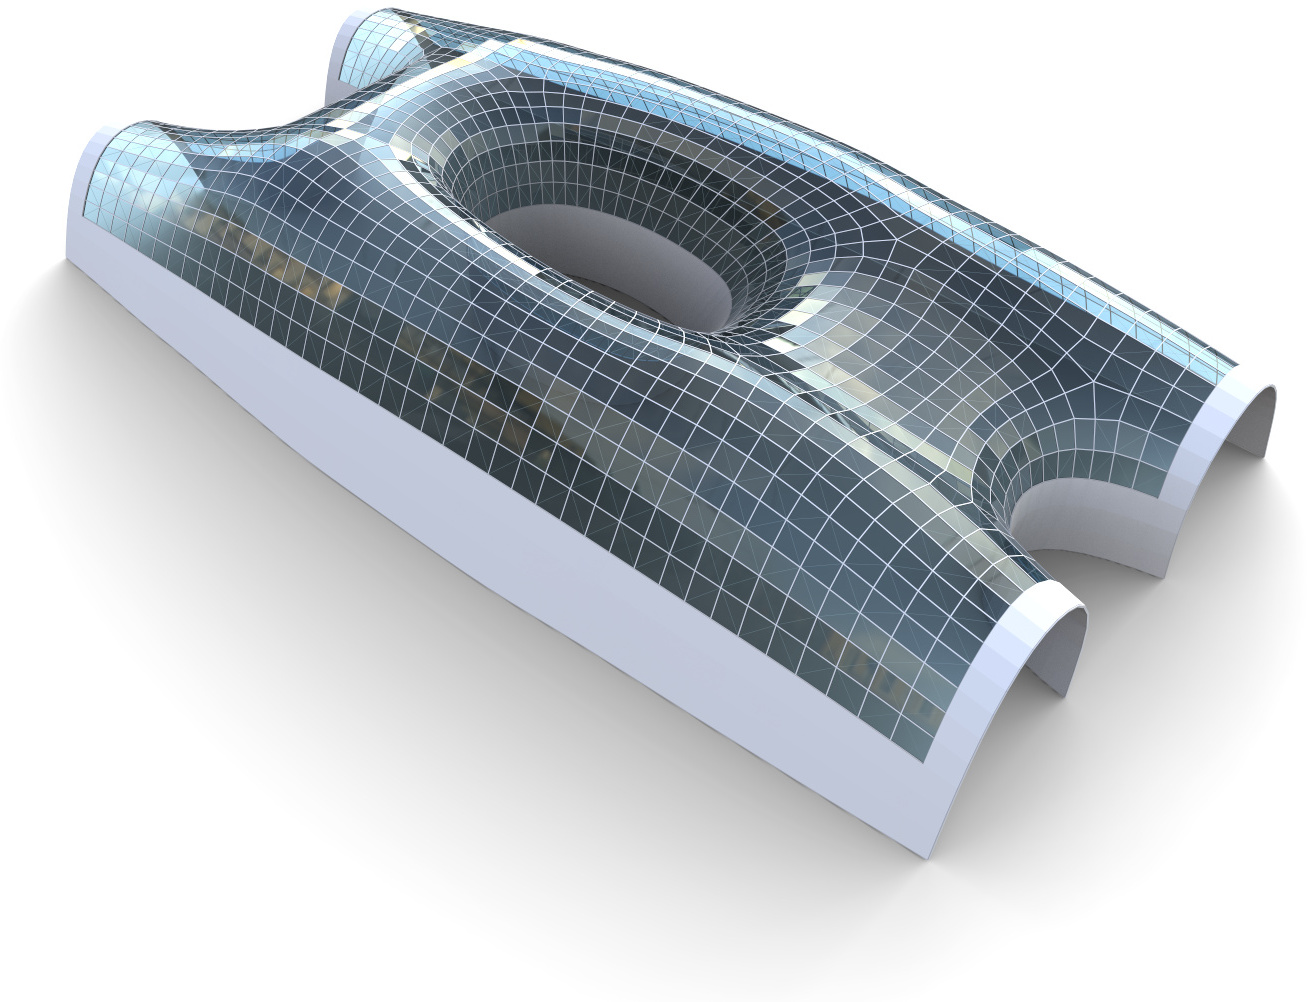
\includegraphics[width=\columnwidth]
		{arch-fig/schneider84.jpg}}}
  \end{overpic}}\vspace*{-1em}

 \begin{minipage}[b]{1.23\columnwidth}
 \caption{Glass as a structural element can support stresses up to, say,
30\,MPa. We propose steel\slash glass constructions which utilize the
structural properties of glass by first solving for a self\dash supporting
thrust network such that forces do not exceed the maximum values, and
subsequent remeshing of this surface by a planar quad mesh (not
necessarily self\dash supporting itself). Since this surface is very
close to a self\dash supporting shape, joints will experience low bending
and torsion moments.}\label{fig:structural}
	\end{minipage}
	\hfill
	\end{figure*}


\bibliographystyle{acmsiggraph}

	%\let\otb=\thebibliography
	%\def\thebibliography#1{\otb{#1}\itemsep-2pt}

\bibliography{selfsupporting}


\end{document}
